\section{三角形五心}
\subsection{外心}

\begin{definition}[外心]
    三角形外接圆的圆心简称为三角形的外心,通常使用O表示。
\end{definition}

\begin{figure}[htbp]
    \centering
    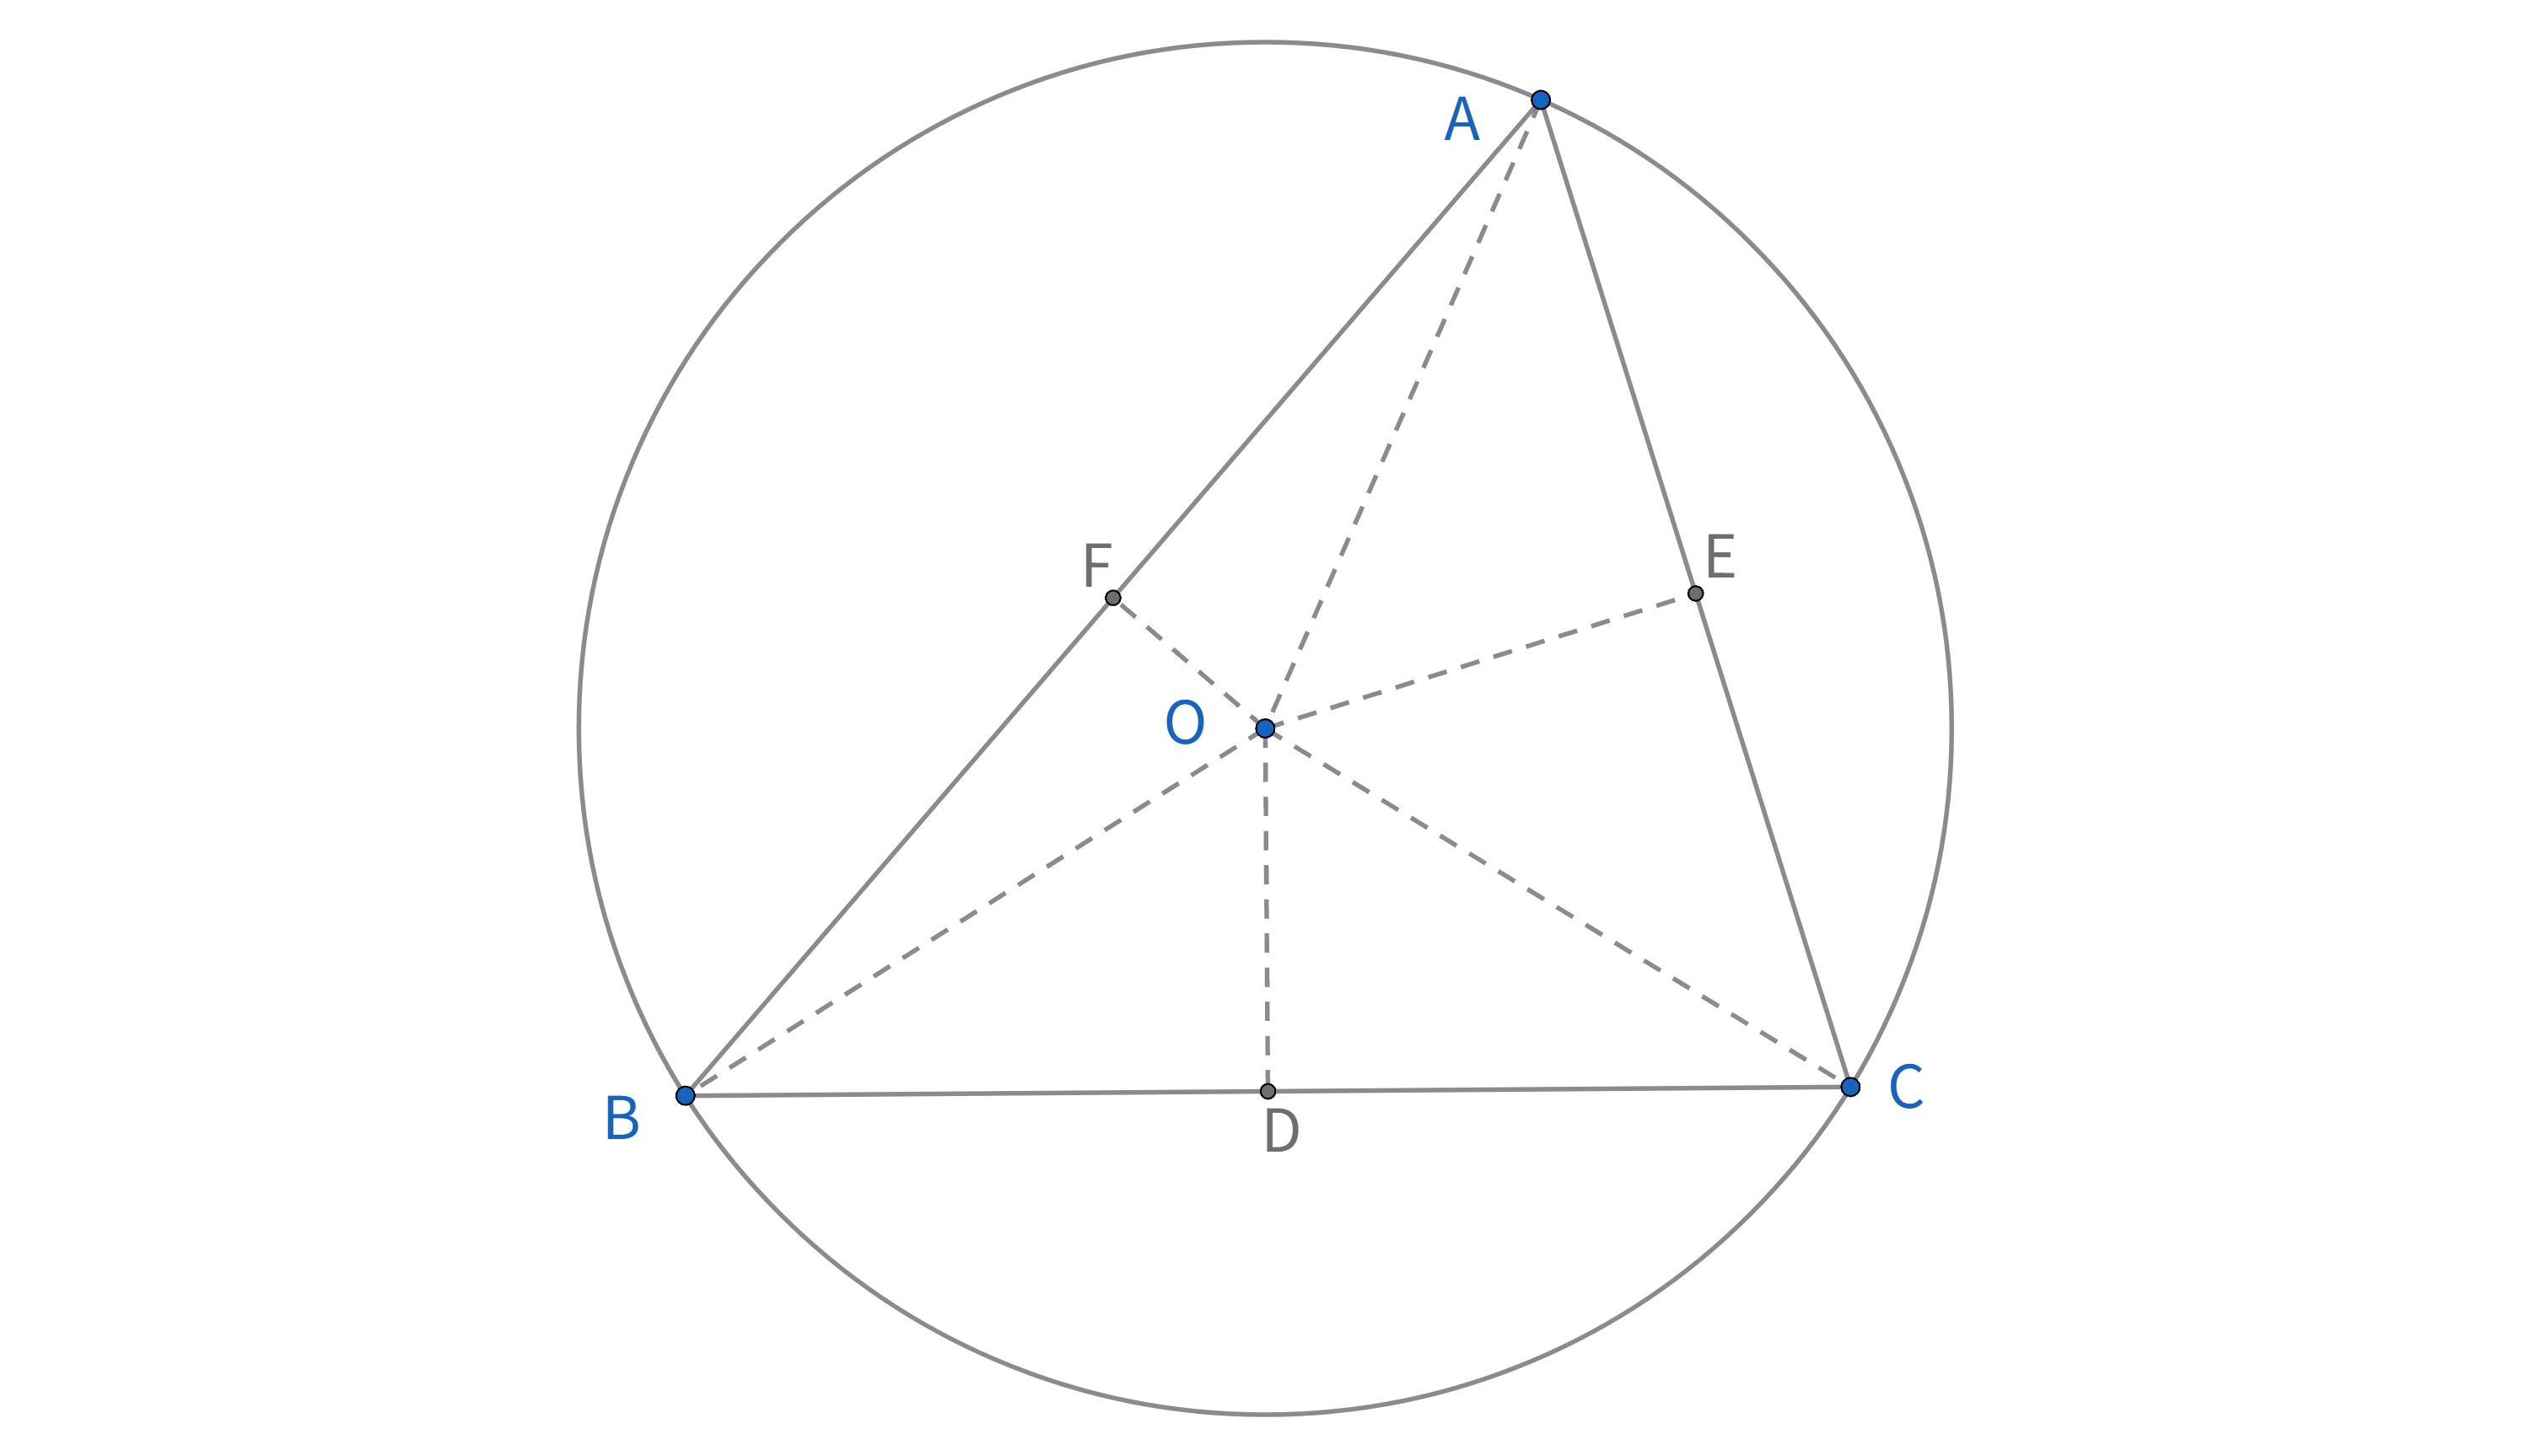
\includegraphics[width=\linewidth]{figures/正弦定理.png}
    \caption{外接圆}
\end{figure}

\begin{proposition}[外心性质]
    三角形外心具有如下性质。
    
    (1) 三角形的外心是三条边中垂线的交点。

    (2) 平面内一点是三角形外心的充分必要条件为:该点到三顶点的距离相等。

    (3) 平面内一点O是三角形$\triangle ABC$外心的充分必要条件为:
    $$\angle BOC = 2A,\quad \angle COA = 2B,\quad \angle AOB =2\angle C.$$

    (4) $BC=2R\sin A,\quad AC =2R\sin B,\quad AC=2R\sin C.$

    (5) 锐角三角形的外心在形内,直角三角形的外心为斜边中点,钝角三角形的外心在形外。
\end{proposition}



%-----------------------------------------------------------------------------------------
\newpage 
\subsection{内心}

\begin{definition}[内心]
    三角形内切圆的圆心简称为三角形的内心,通常使用I表示。
\end{definition}

\begin{figure}[ht]
    \centering
    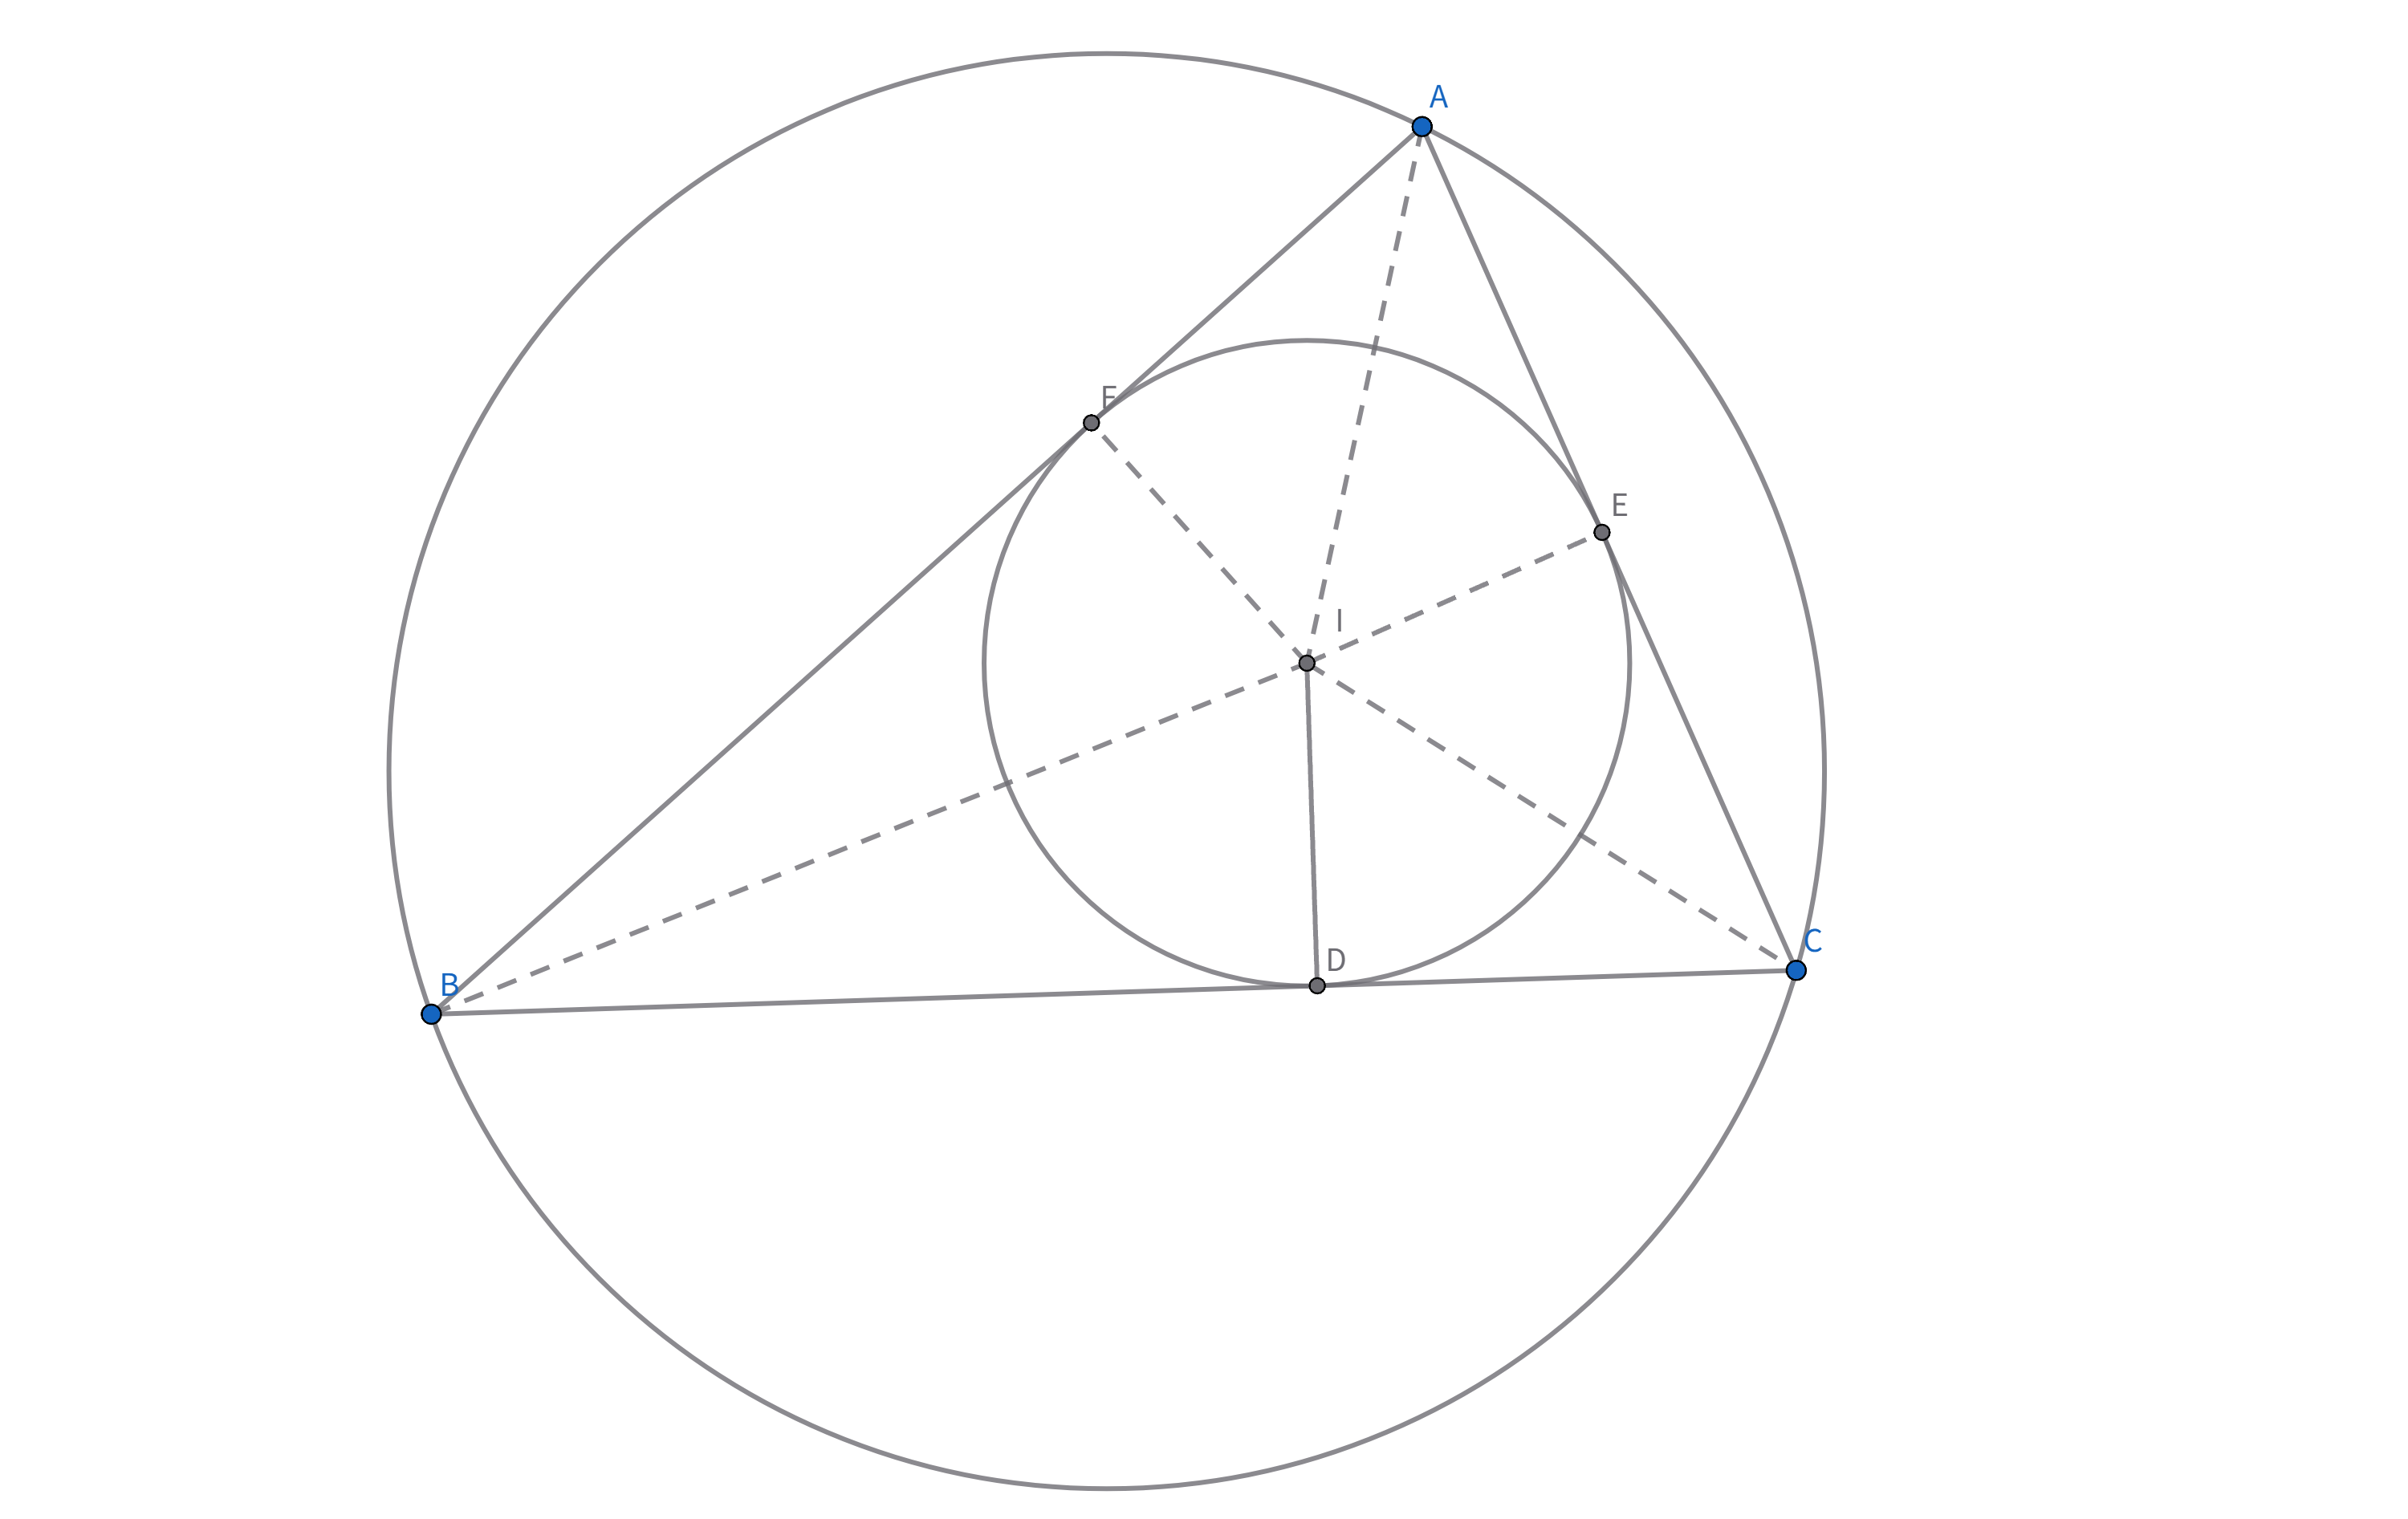
\includegraphics[width=\linewidth]{figures/内心.png}
    \caption{内心}
\end{figure}

\begin{proposition}[内心性质]
    三角形内心具有如下性质。
    
    (1) 三角形的内心是三条内角平分线的交点。

    (2) 内心到三边的距离相等。

    (3) 平面内一点I是三角形$\triangle ABC$内心的充分必要条件为:
    $$\angle BIC = 90^\circ +\frac{1}{2}A,\quad \angle AIC = 90^\circ +\frac{1}{2}B,
    \quad \angle AIB =90^\circ +\frac{1}{2}C.$$

    (4) 设D、E、F分别为内切圆I在BC、CA、AB上的切点,那么
    $$
    ID \perp BC,\quad 
    IE \perp AC, \quad 
    IF \perp AB.$$
    并且切线长度可由三边边长表示:
    $$
    BF=BD=\frac{1}{2}(a+c - b),\quad 
    CD=CE=\frac{1}{2}(a+b - c),\quad 
    AE=AF=\frac{1}{2}(b+c - a).
    $$
\end{proposition}


\begin{theorem}[鸡爪定理]
    对平面内任意$\triangle ABC$,O、I分别为其外心和内心。设AI延长线与圆O相交于D,
    D为$\overset{{\frown}}{BC}$的中点,并且满足
    $$DB=DI=DC.$$
\end{theorem}

\begin{figure}[ht]
    \centering
    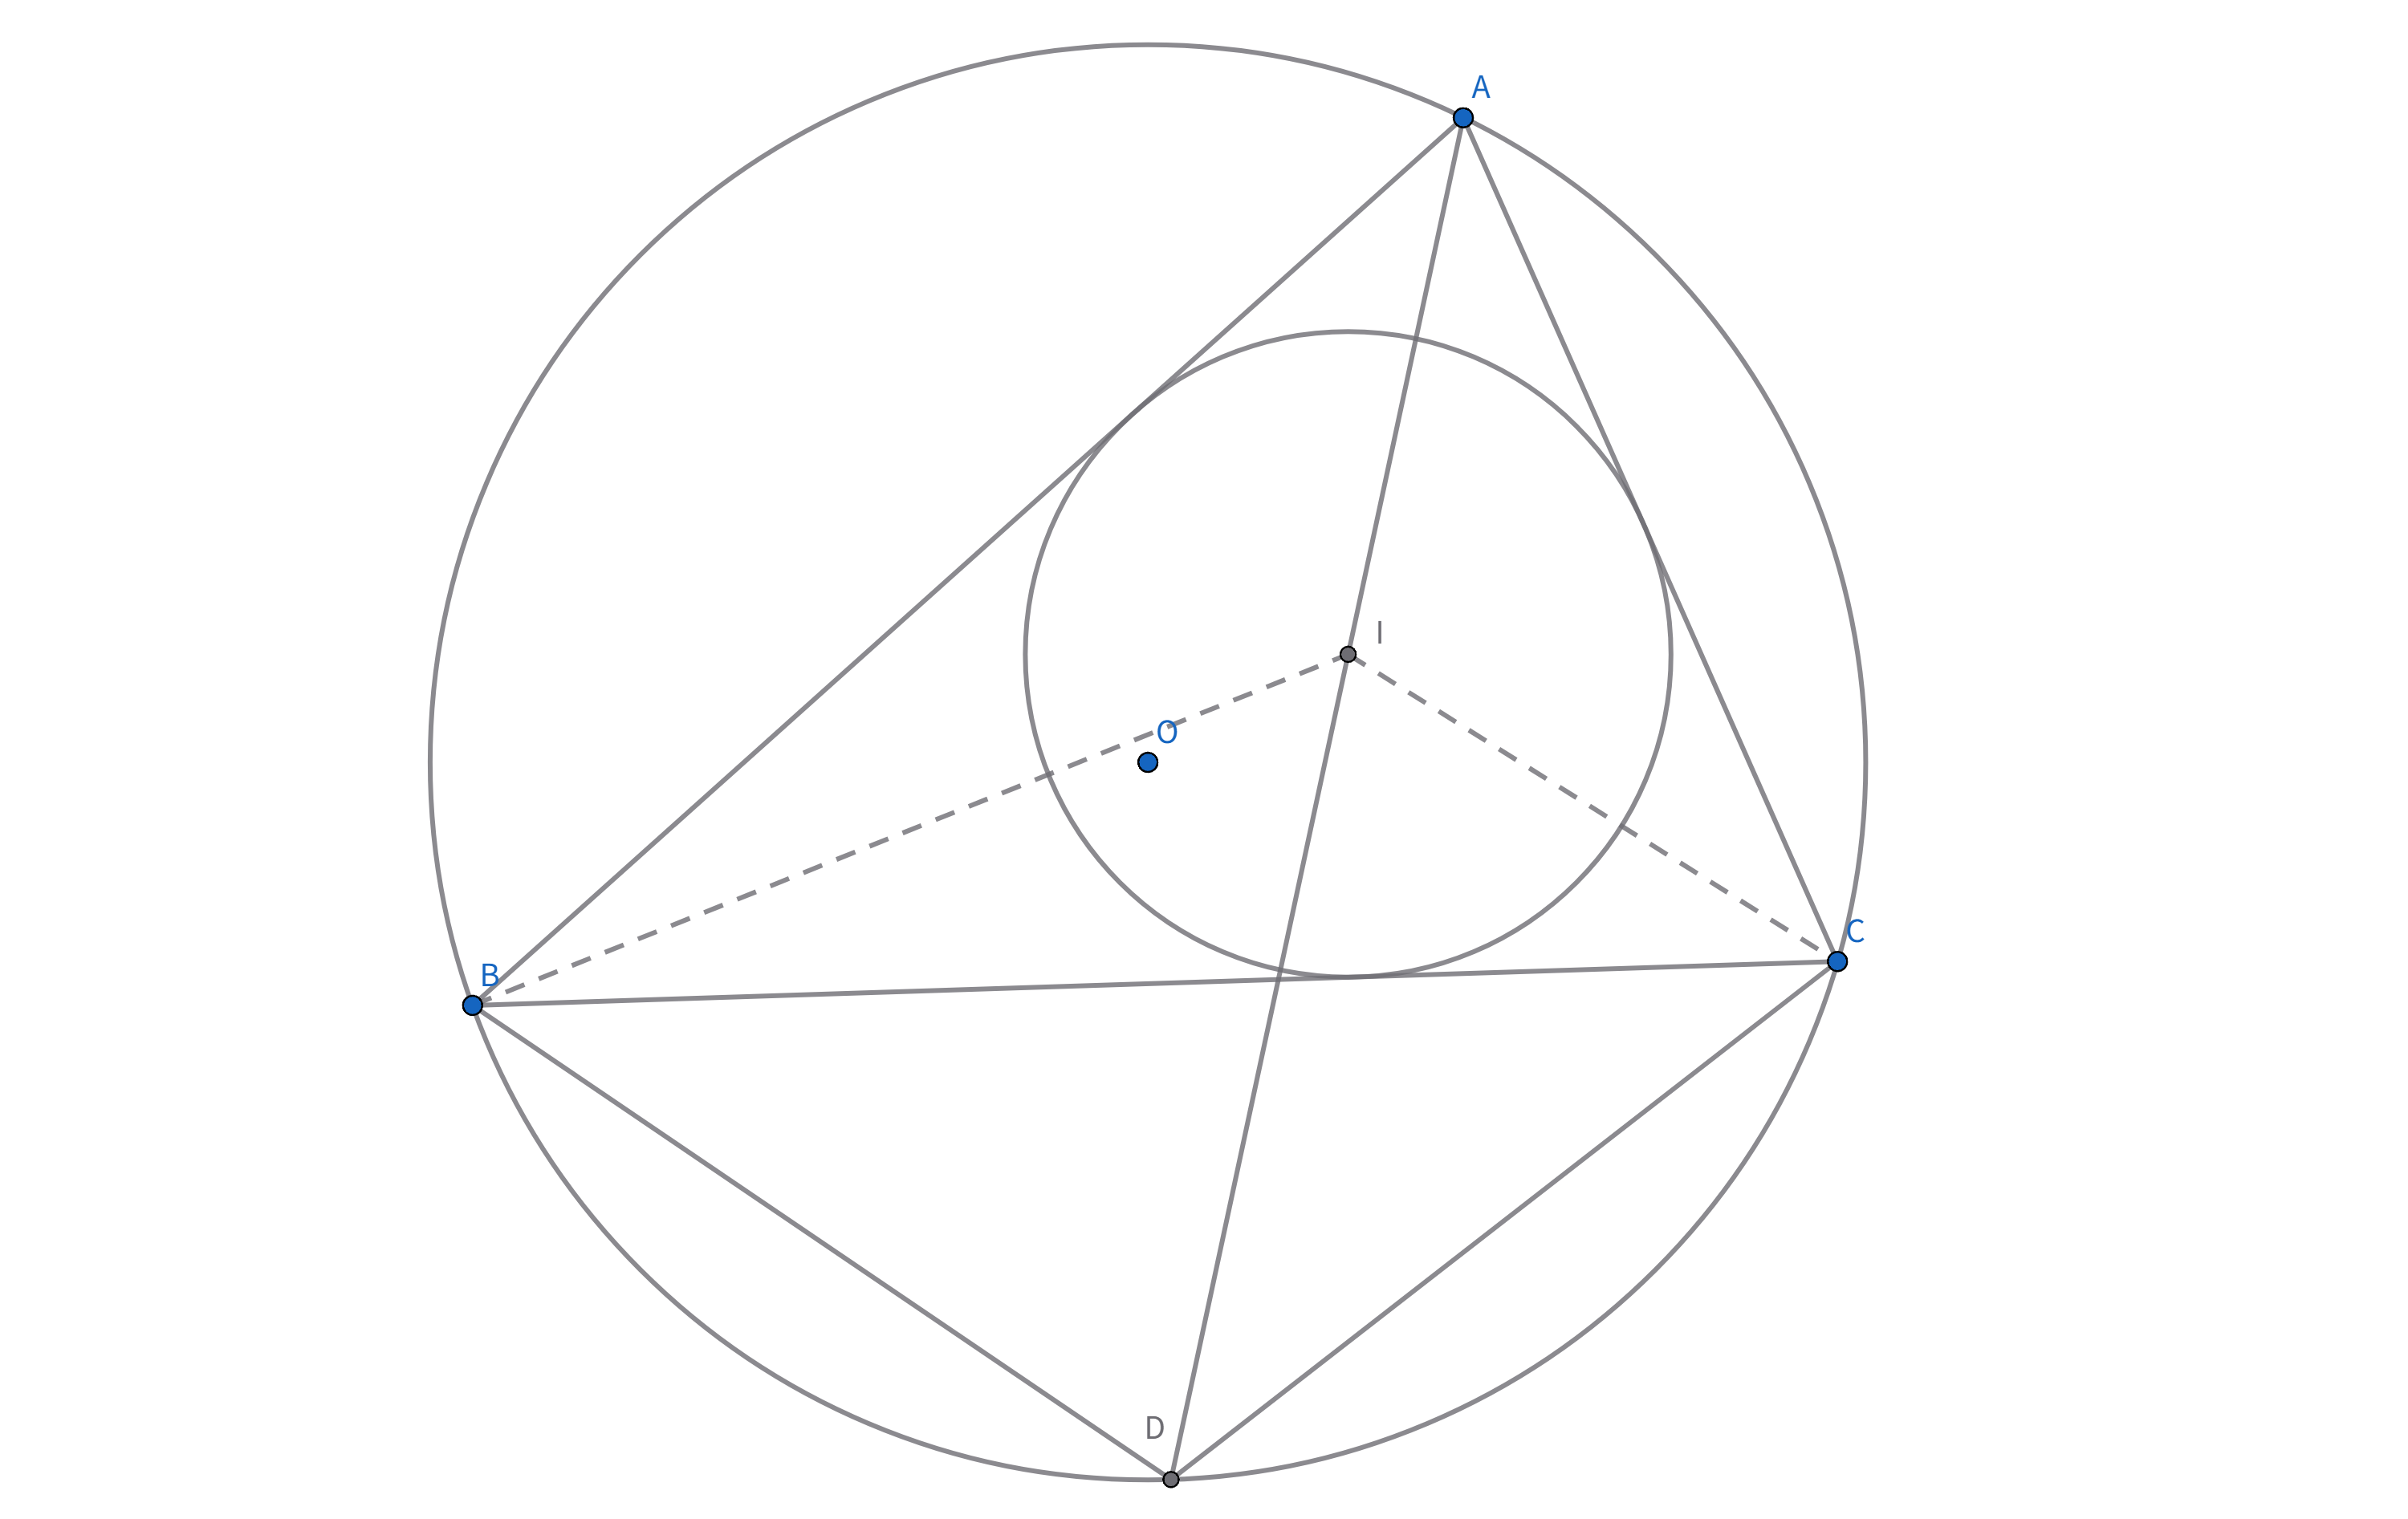
\includegraphics[width=\linewidth]{figures/内心-鸡爪定理.png}
    \caption{鸡爪定理}
\end{figure}





%-----------------------------------------------------------------------------------------
\newpage
\subsection{垂心}
\begin{definition}[垂心]
    三角形三边上高线的交点称为三角形的垂心,通常使用H表示。
\end{definition}

\begin{figure}[htbp]
    \centering
    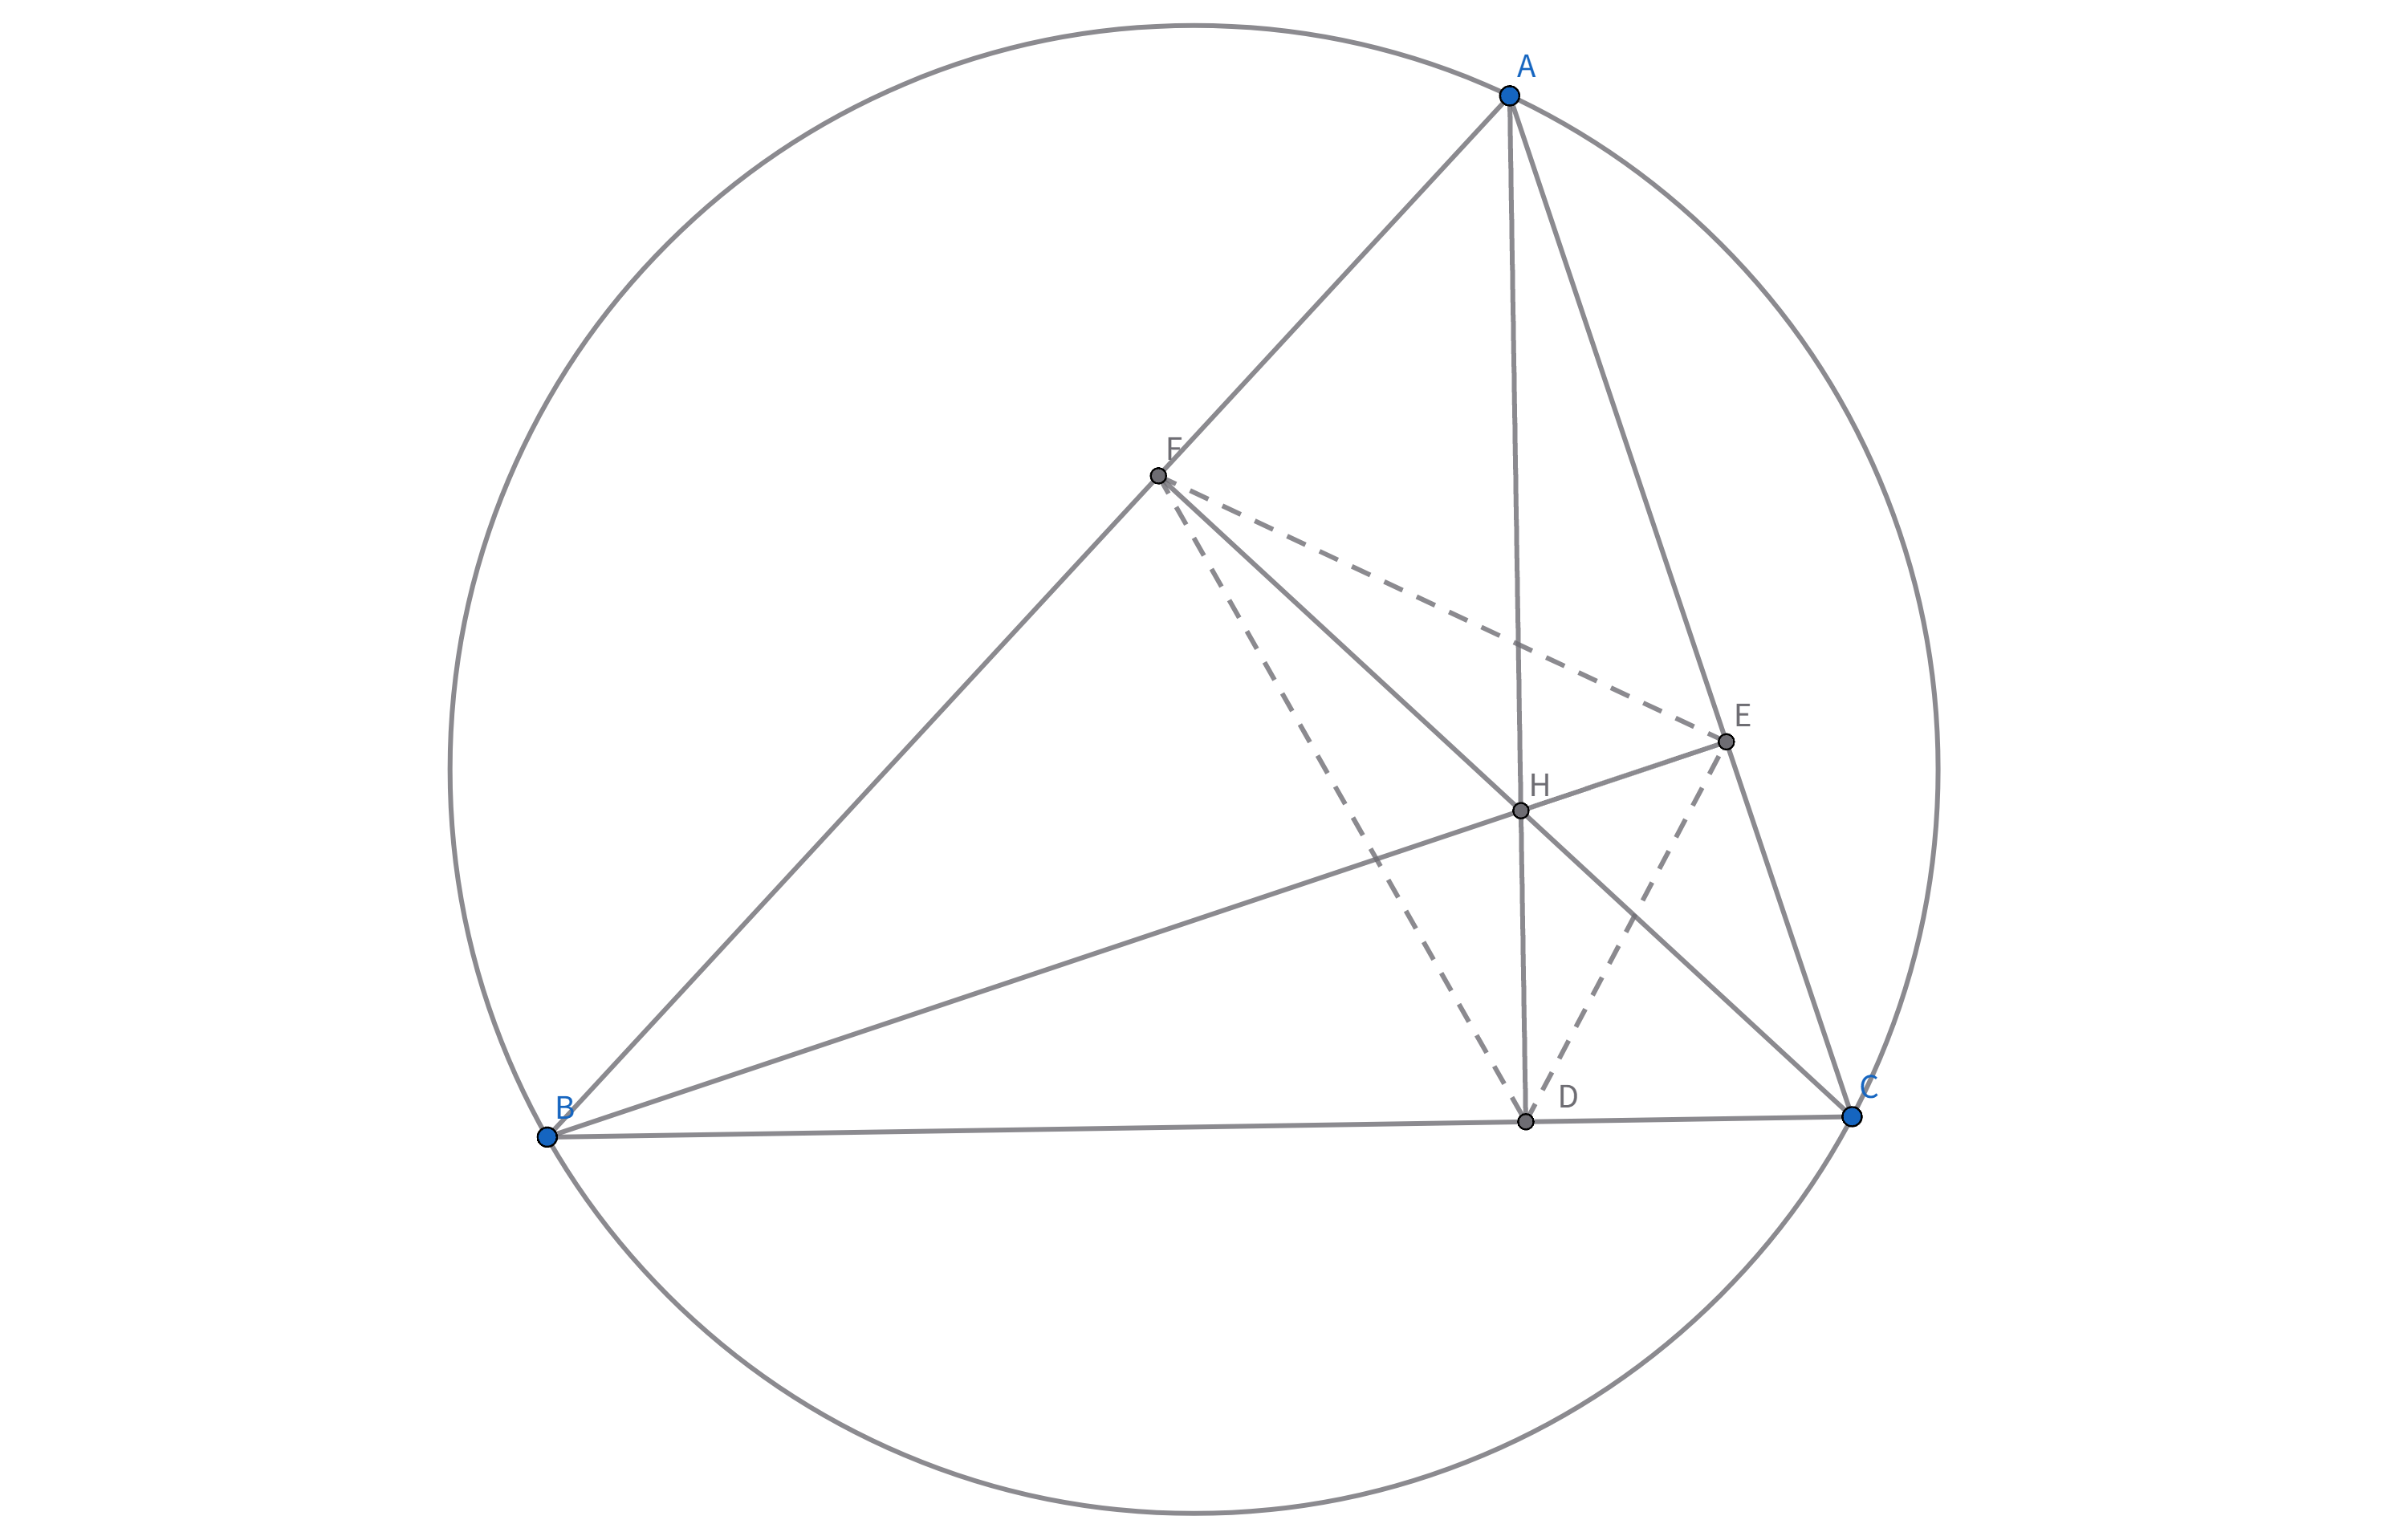
\includegraphics[width=\linewidth]{figures/垂足三角形.png}
    \caption{垂心}
\end{figure}

\begin{proposition}[垂心性质]
    三角形垂心具有如下性质。

    (1) 若H是三角形$\triangle ABC$的垂心,则
    $$\angle BHC = 180^\circ - A,\quad \angle AHC = 180^\circ - B,\quad \angle AHB =180^\circ - C.$$

    (2) 设$\triangle ABC$的外接圆半径为R,则
    $$AH=2R\cdot |\cos A|,\quad
    BH=2R\cdot |\cos B|,\quad
    CH=2R\cdot |\cos C|.$$

    (3) 垂心H为垂足$\triangle DEF$的内心。


    (4) 锐角三角形的垂心在形内,直角三角形的垂心在直角顶点,钝角三角形的垂心在形外。

    (5) 若H为三角形$\triangle ABC$的垂心,则A、B、C、H四点中任意一点是其余三点构成的三角形的垂心,称A、B、C、H为垂心组。
\end{proposition}



\newpage 
\begin{figure}[htbp]
    \centering
    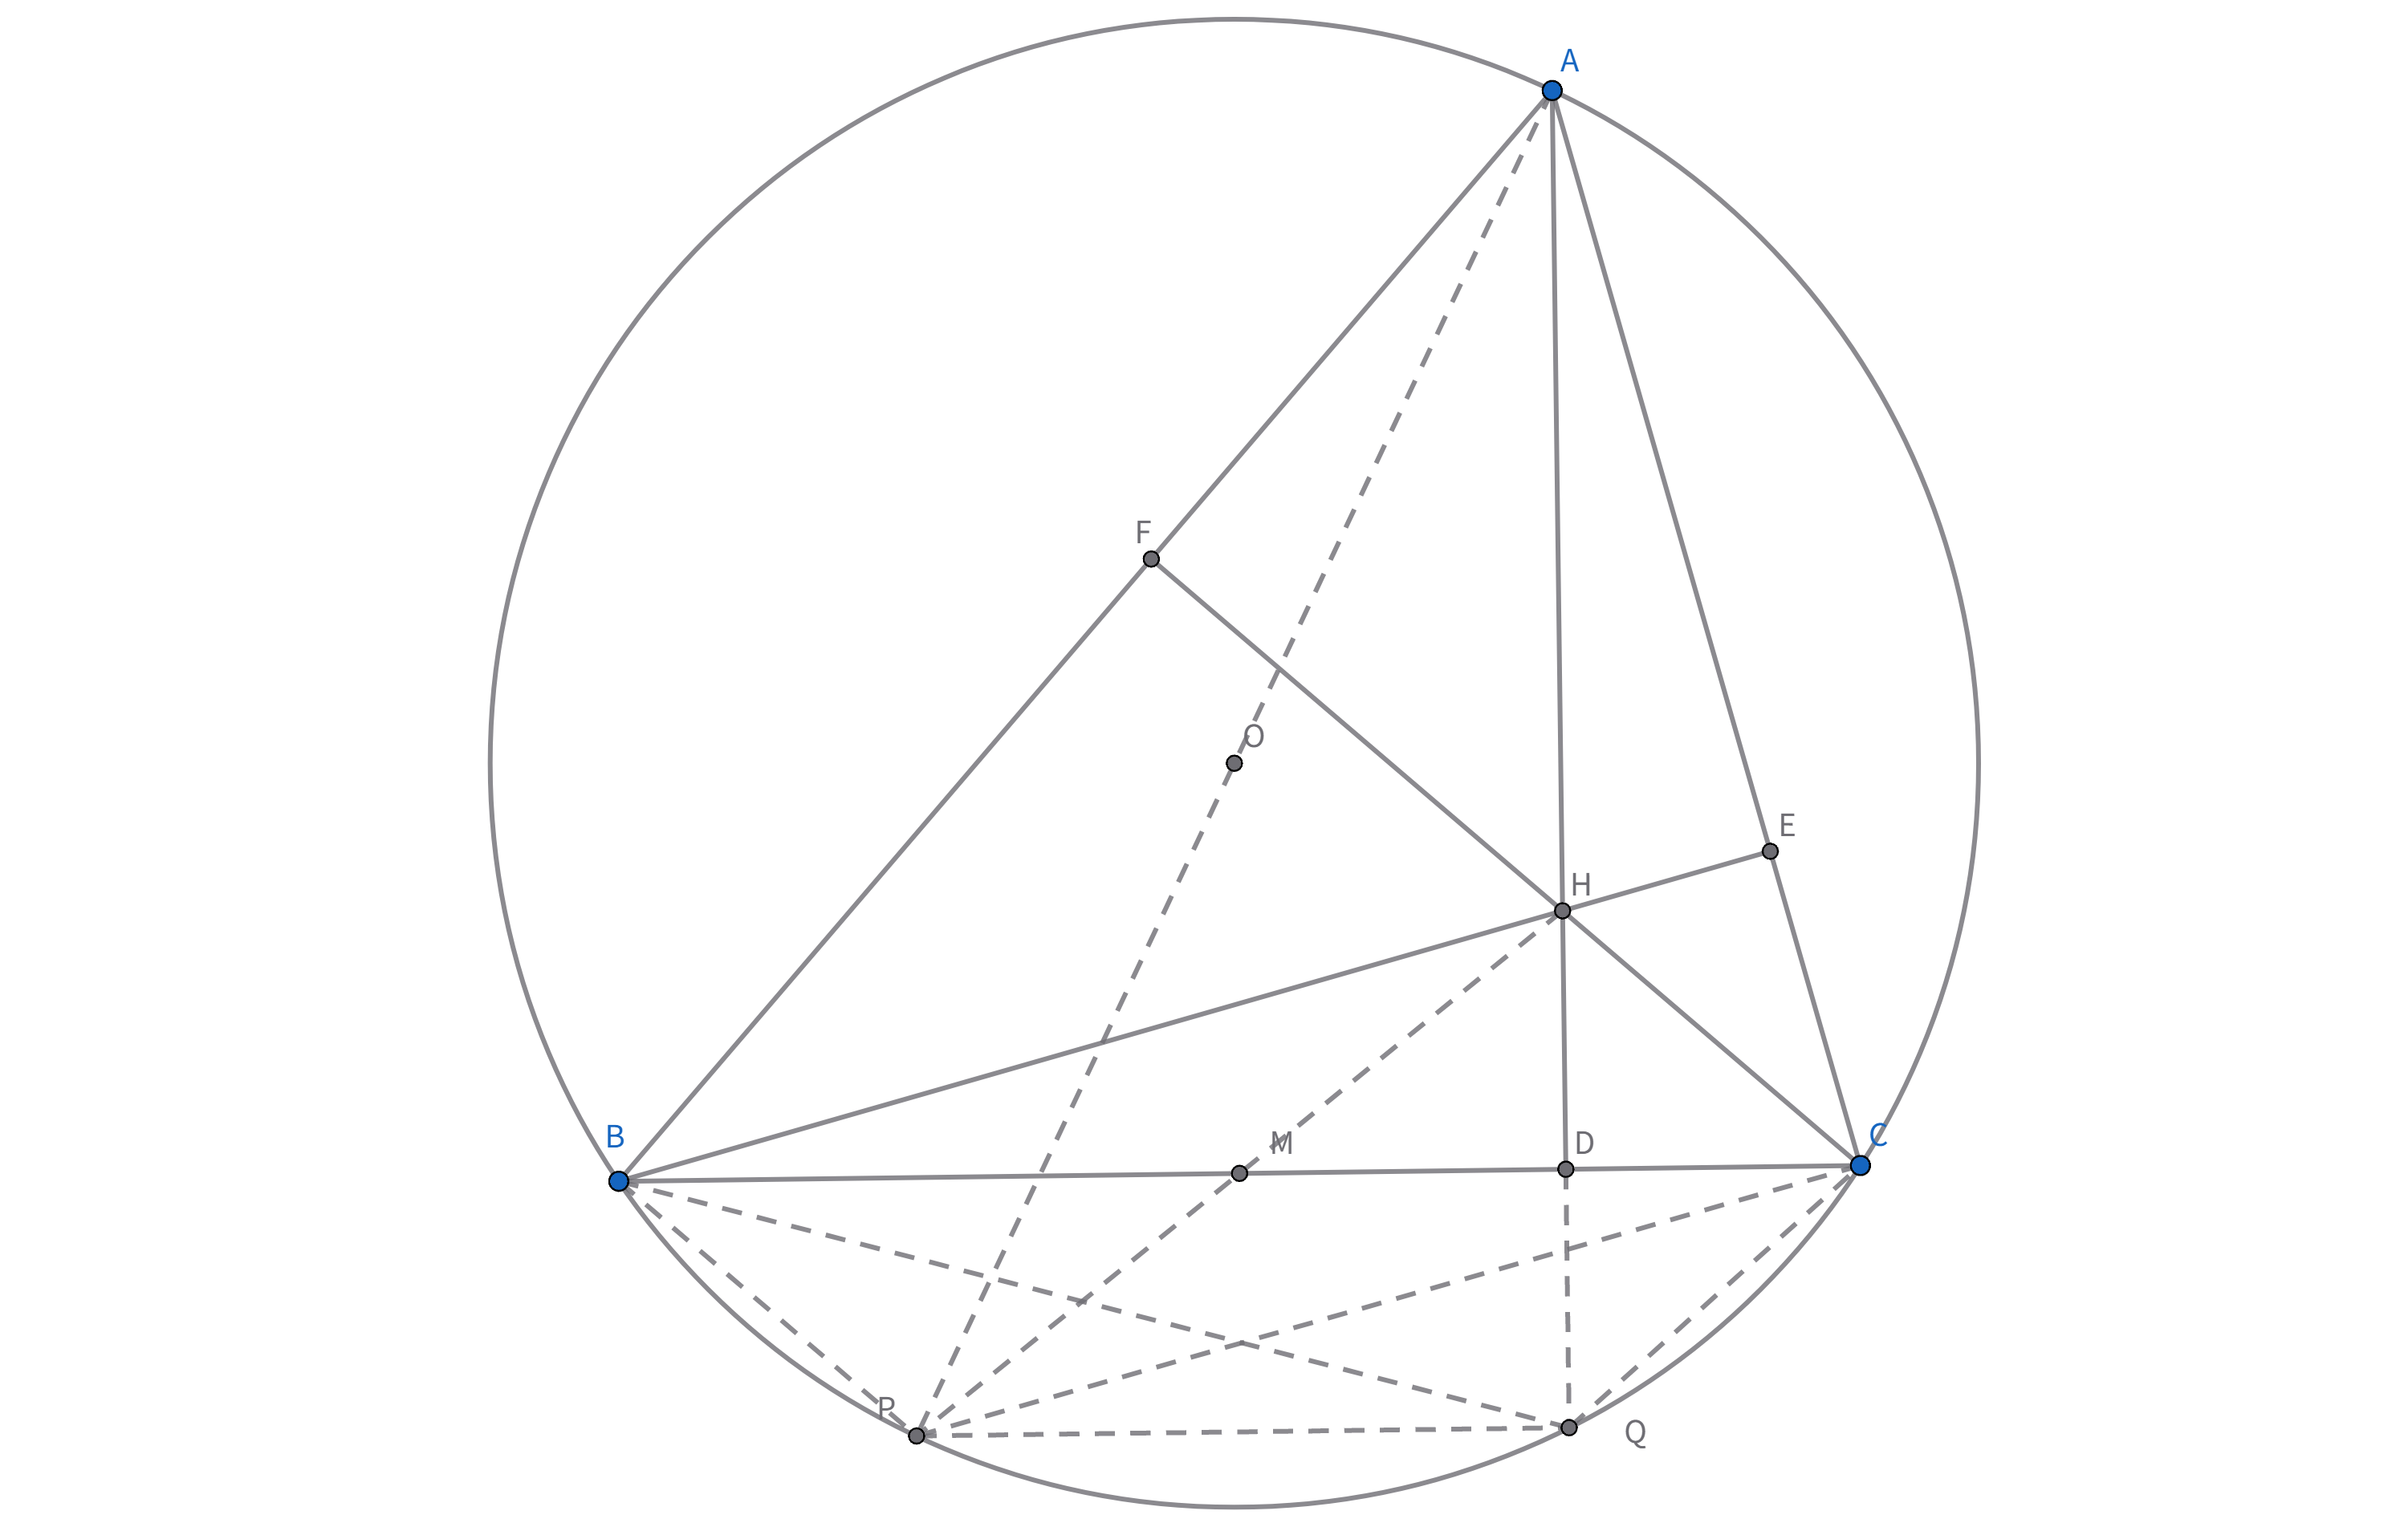
\includegraphics[width=0.7\linewidth]{figures/垂心性质.png}
    \caption{垂心性质}
\end{figure}

\begin{theorem}
    H为锐角$\triangle ABC$所在平面内的一点,H为$\triangle ABC$垂心的充分必要条件是下列条件之一成立:

    (1) $\angle HAB = \angle HCB, \quad \angle HBC = \angle HAC.$
    

    (2) H关于三边的对称点均在$\triangle ABC$的外接圆上。

    (3) H关于三边中点的对称点均在$\triangle ABC$的外接圆上。

    (4) $\triangle ABC,\triangle ABH,\triangle BCH, \triangle ACH$的外接圆是等圆。

    (5) (卡诺定理)$\triangle ABC$任一顶点到垂心H的距离,等于外心O到对边距离的2倍,即$AH = 2OM.$

    (6) H是外心O关于$\triangle ABC$的等角共轭点,即
    $$\angle BAO = \angle CAH, \quad 
    \angle ACO = \angle BCH, \quad 
    \angle CBO = \angle ABH.$$
\end{theorem}

\begin{figure}[htbp]
    \centering
    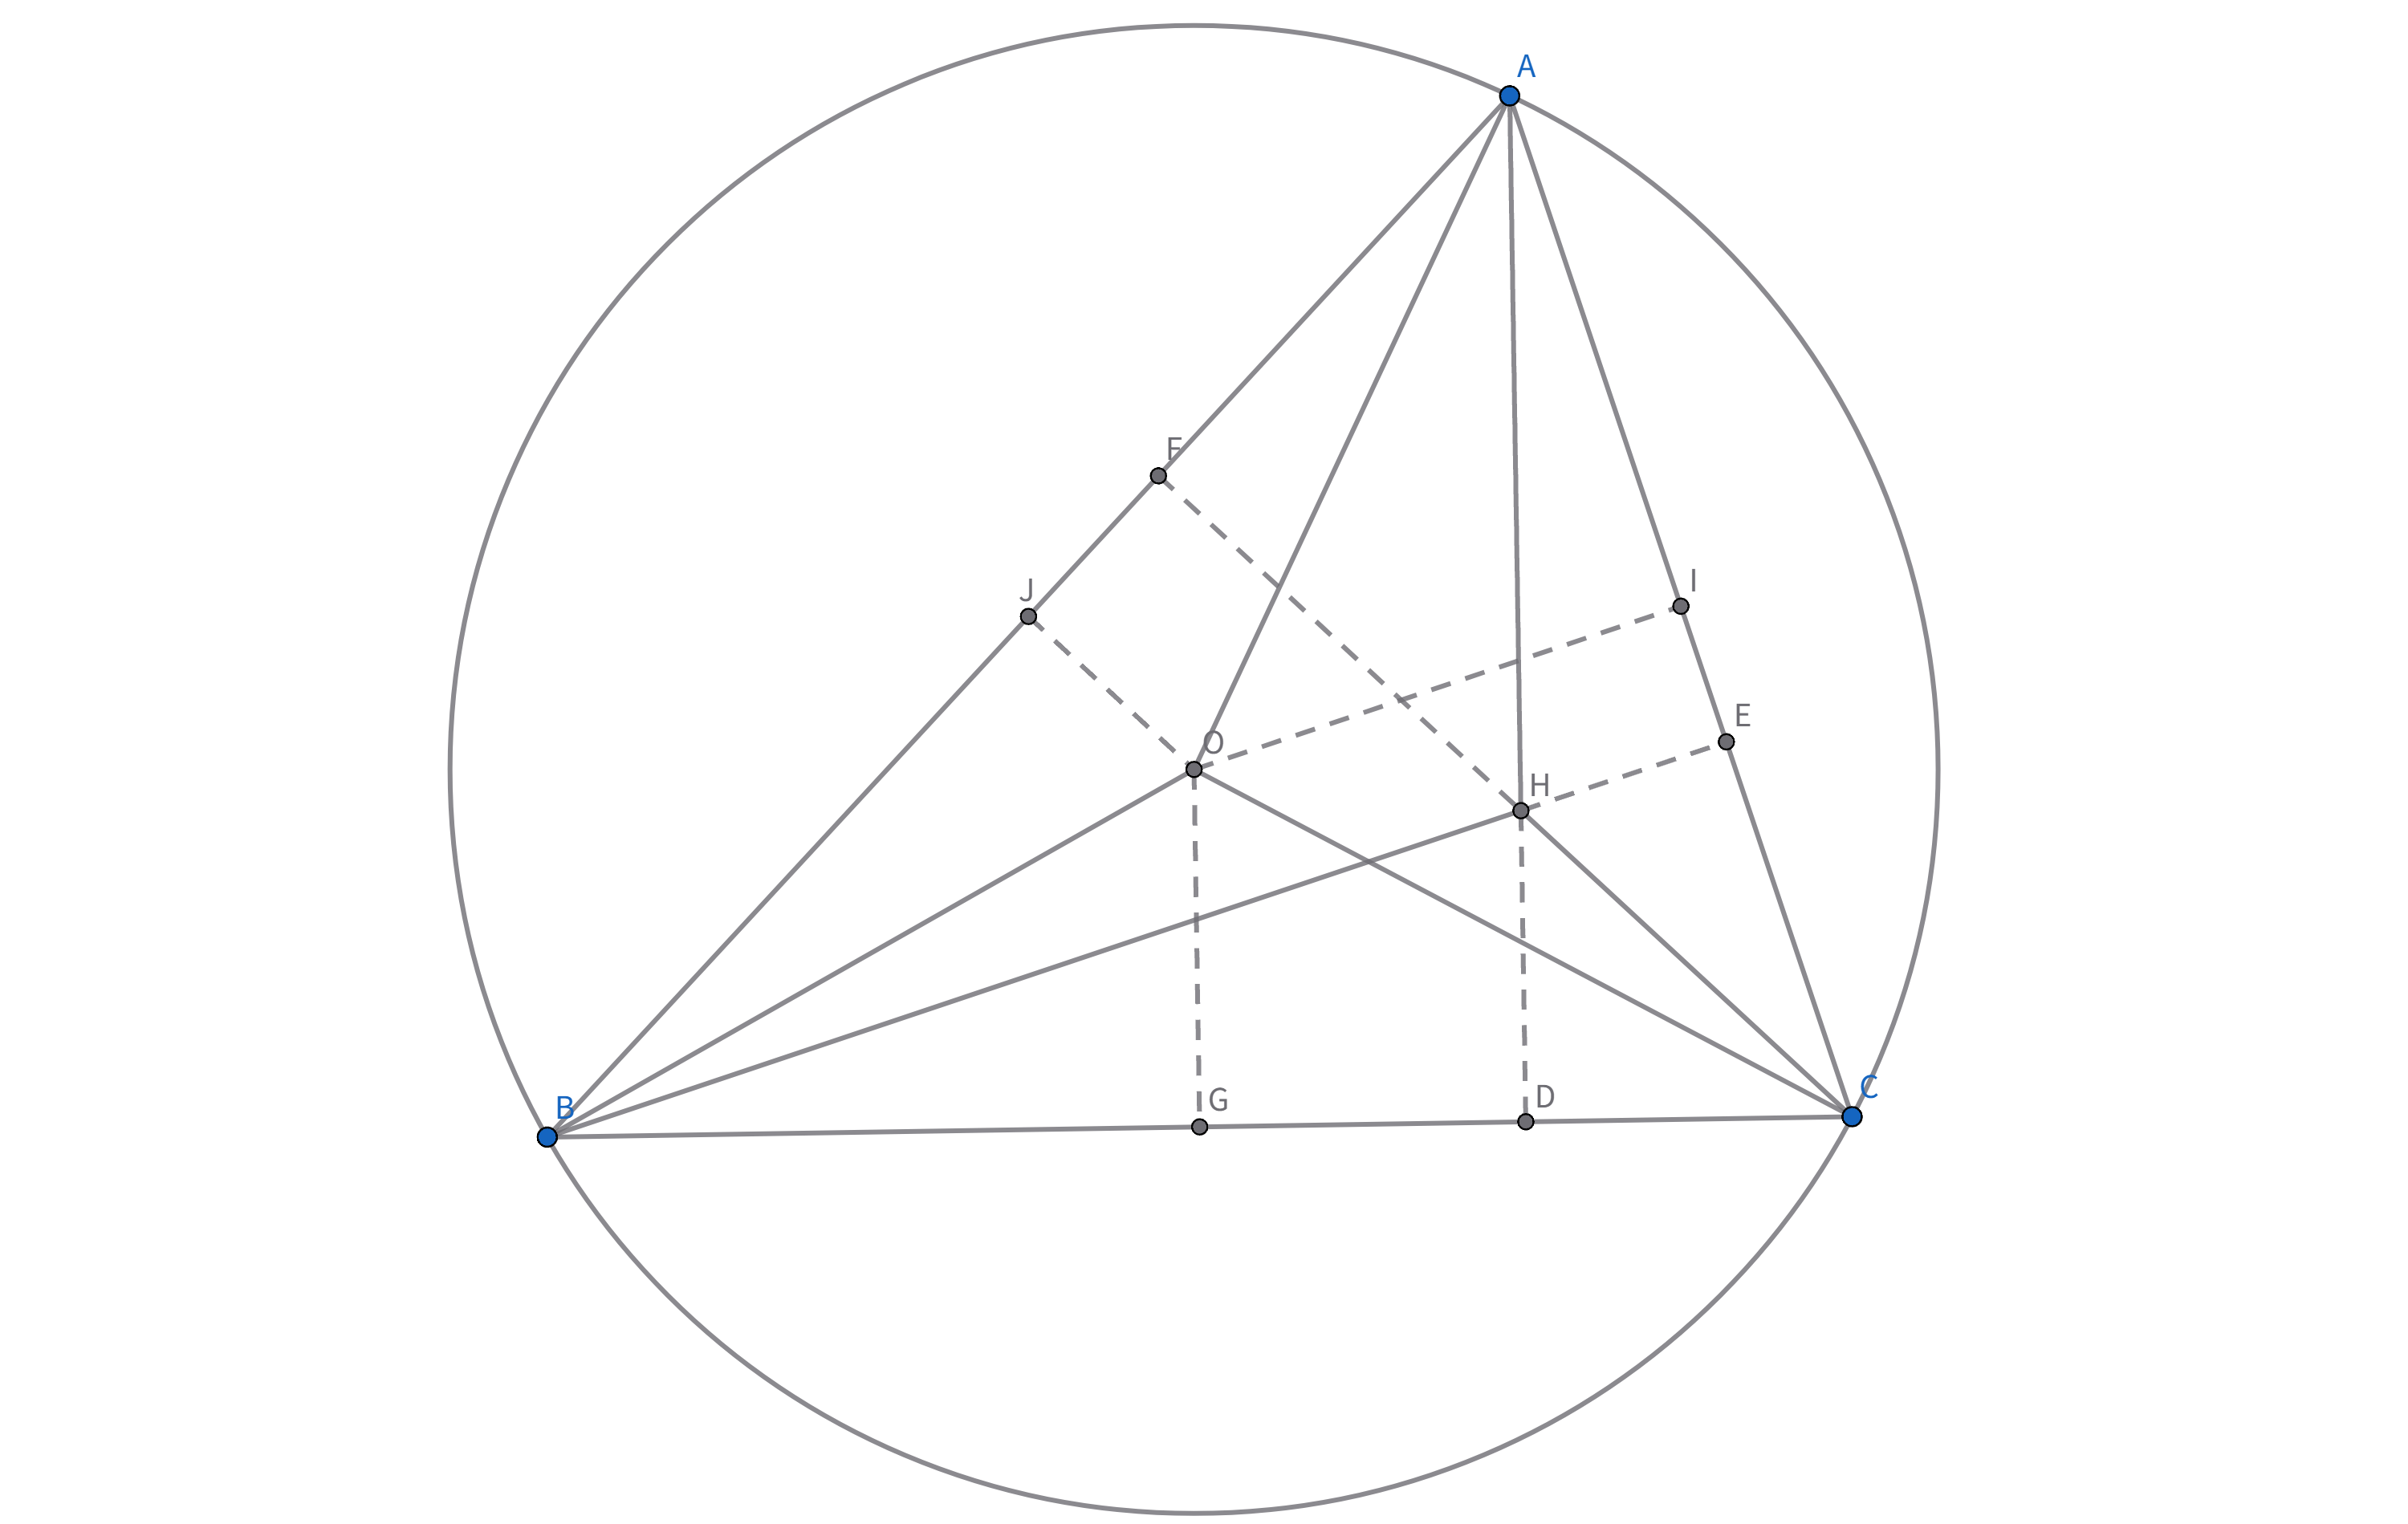
\includegraphics[width=0.7\linewidth]{figures/外心垂心等角共轭.png}
    \caption{外心垂心等角共轭}
\end{figure}


%-----------------------------------------------------------------------------------------
\newpage
\subsection{重心}
\begin{definition}[重心]
    三角形三条中线的交点称为三角形的重心,通常使用G表示。
\end{definition}

\begin{figure}[ht]
    \centering
    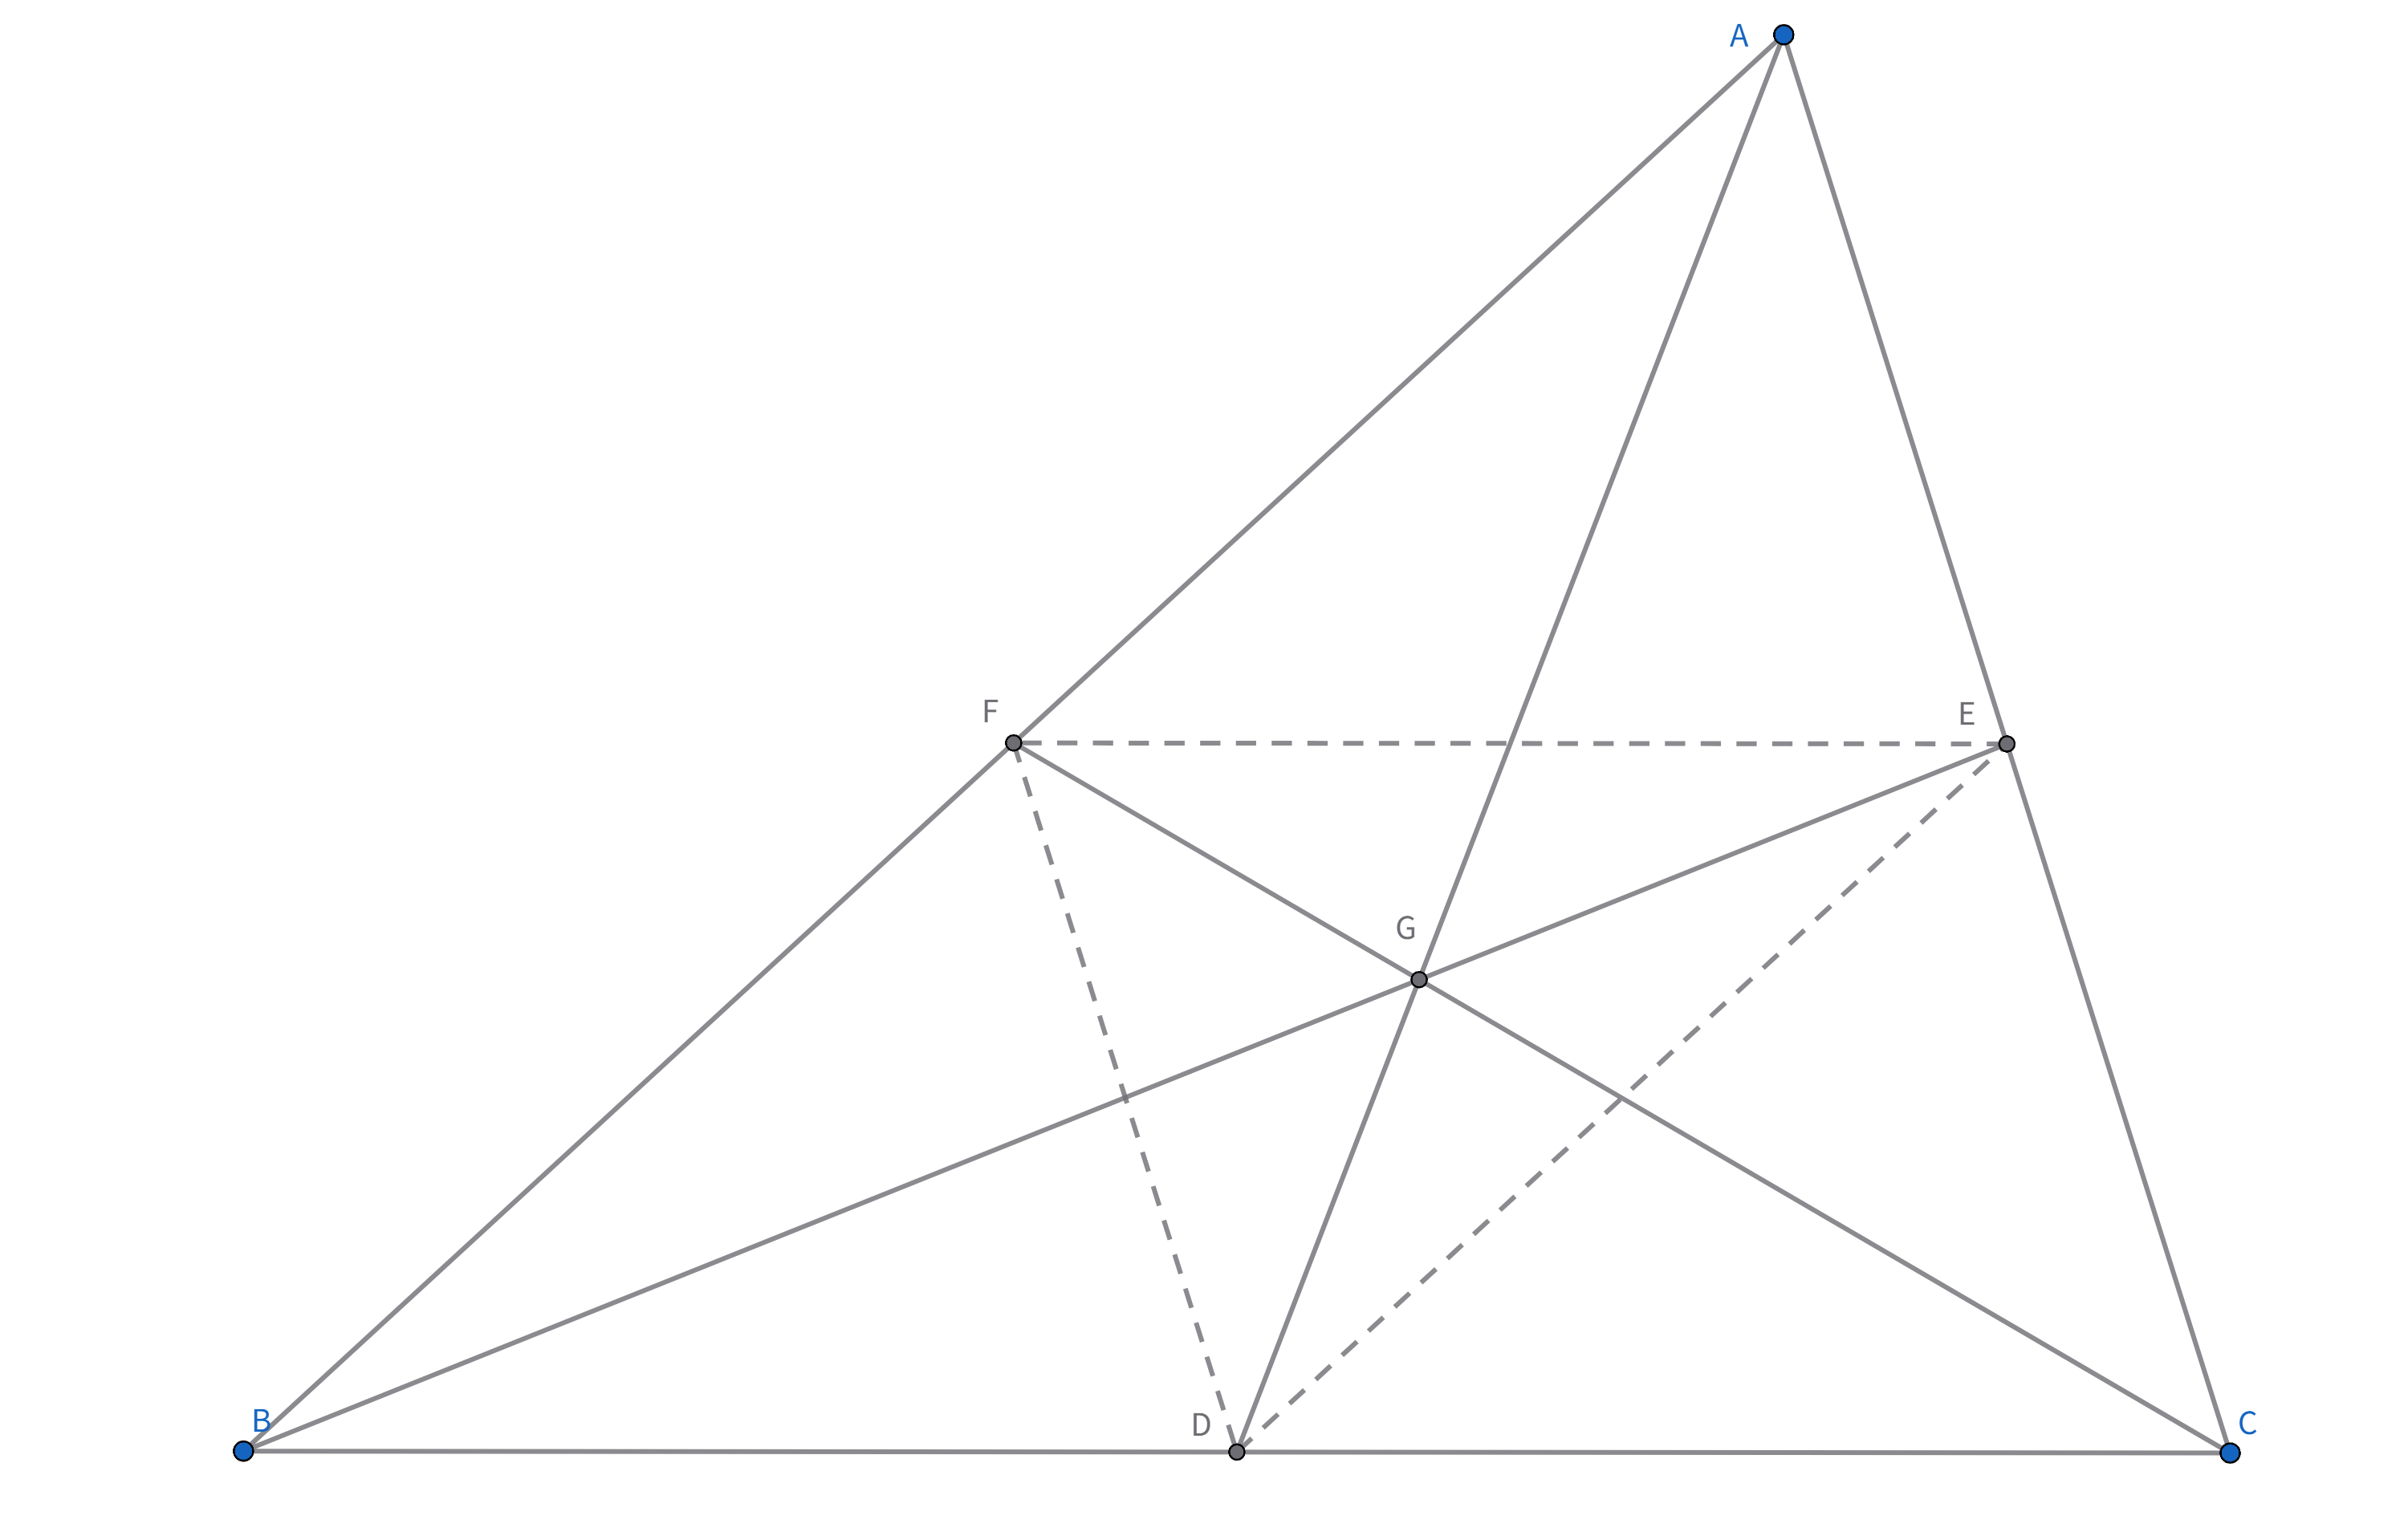
\includegraphics[width=\linewidth]{figures/重心.png}
    \caption{重心}
\end{figure}

\begin{proposition}[重心性质]
    三角形重心具有如下性质。
    
    (1) 重心G为三条中线的三等分点,满足
    $$AG=2GD,\quad 
    BG=2GE,\quad
    CG=2GF.$$

    (2) 三边与重心组成的三角形面积相等,即
    $$S_{\triangle ABG} = S_{\triangle BCG}=S_{\triangle CAG}.$$

    (3) $\triangle ABC \sim \triangle DEF$,且相似比为2.

    (4) $2AD^2=AB^2+AC^2-\frac{1}{2}BC^2.$
\end{proposition}
%-----------------------------------------------------------------------------------------
\newpage
\subsection{旁心}
\begin{definition}[旁心]
    与三角形一边外侧相切,又与另两边的延长线相切的圆叫做三角形的旁切圆,通常用J,或者$I_a,I_b,I_c$表示。    
\end{definition}

% \begin{figure}[htbp]
%     \centering
%     \hfill % 添加一些水平间距
%     \begin{minipage}[t]{0.45\textwidth}
%         \centering
%         \includegraphics[width=\linewidth]{figures/旁心 (1).png}
%         \caption{旁心}
%     \end{minipage}
%     \hfill % 添加一些水平间距
%     \begin{minipage}[t]{0.45\textwidth}
%         \centering
%         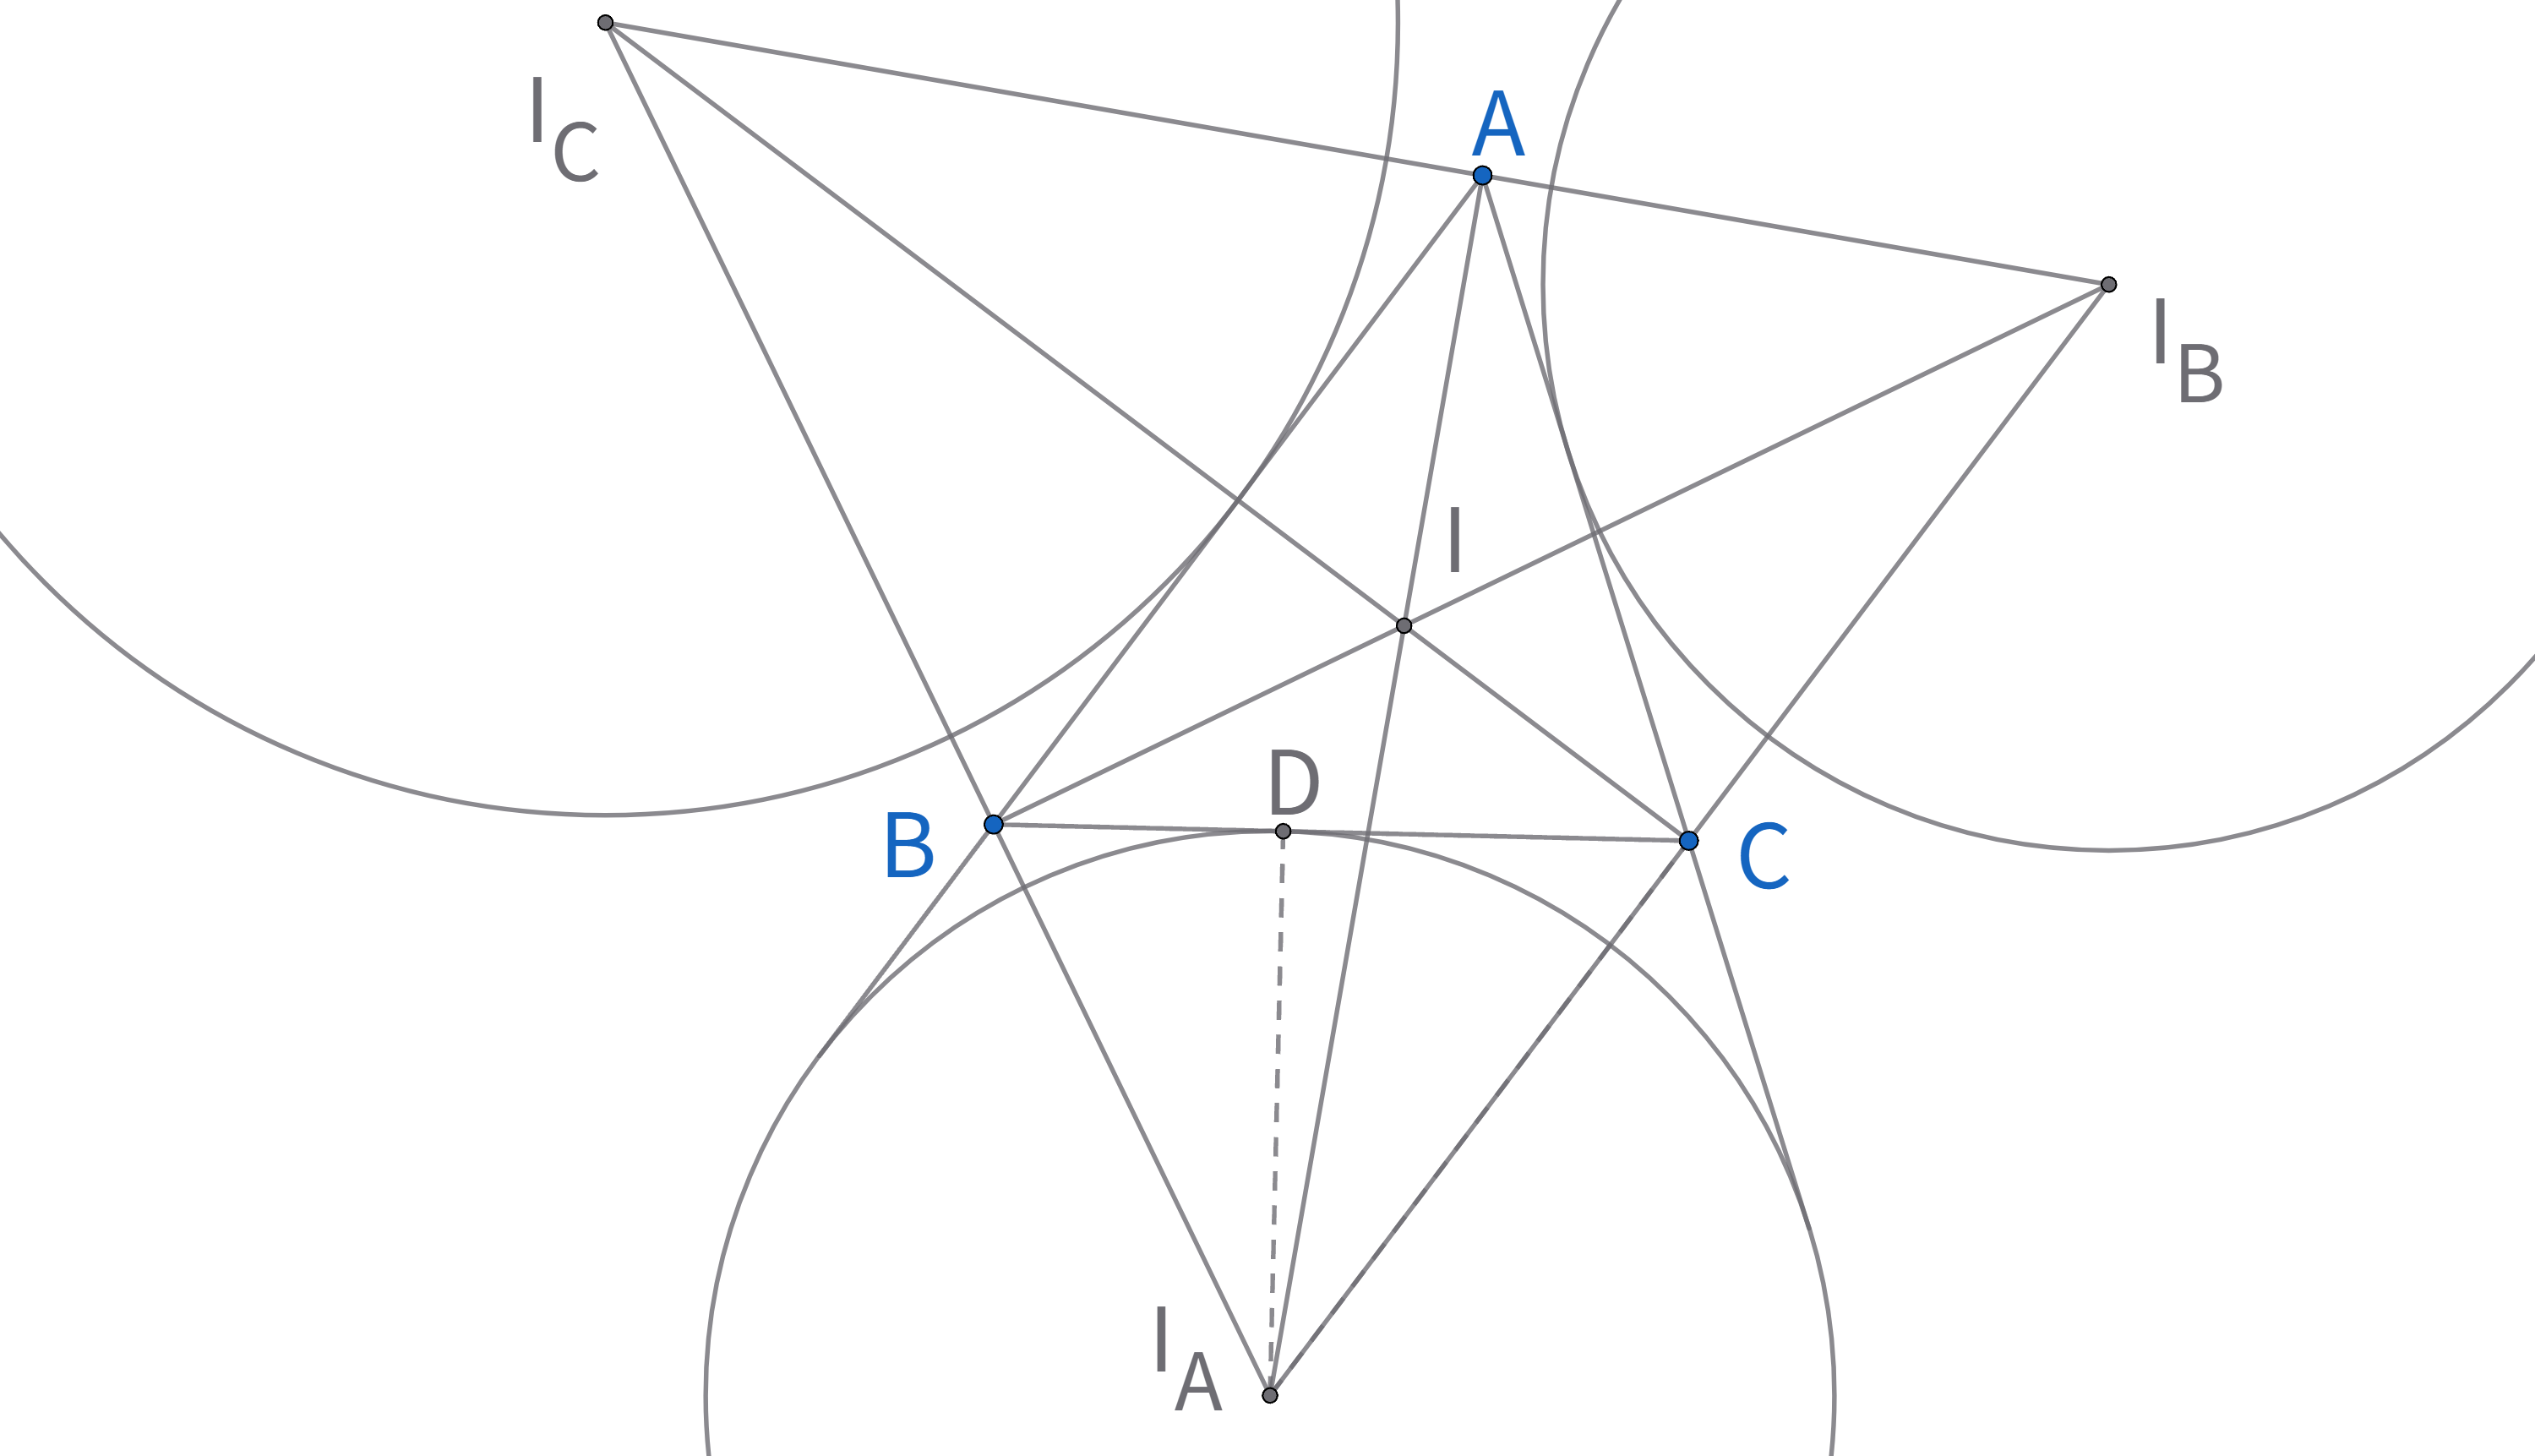
\includegraphics[width=\linewidth]{figures/旁心三角形.png}
%         \caption{旁心三角形}
%     \end{minipage}
% \end{figure}


\begin{figure}[htbp]
    \centering
    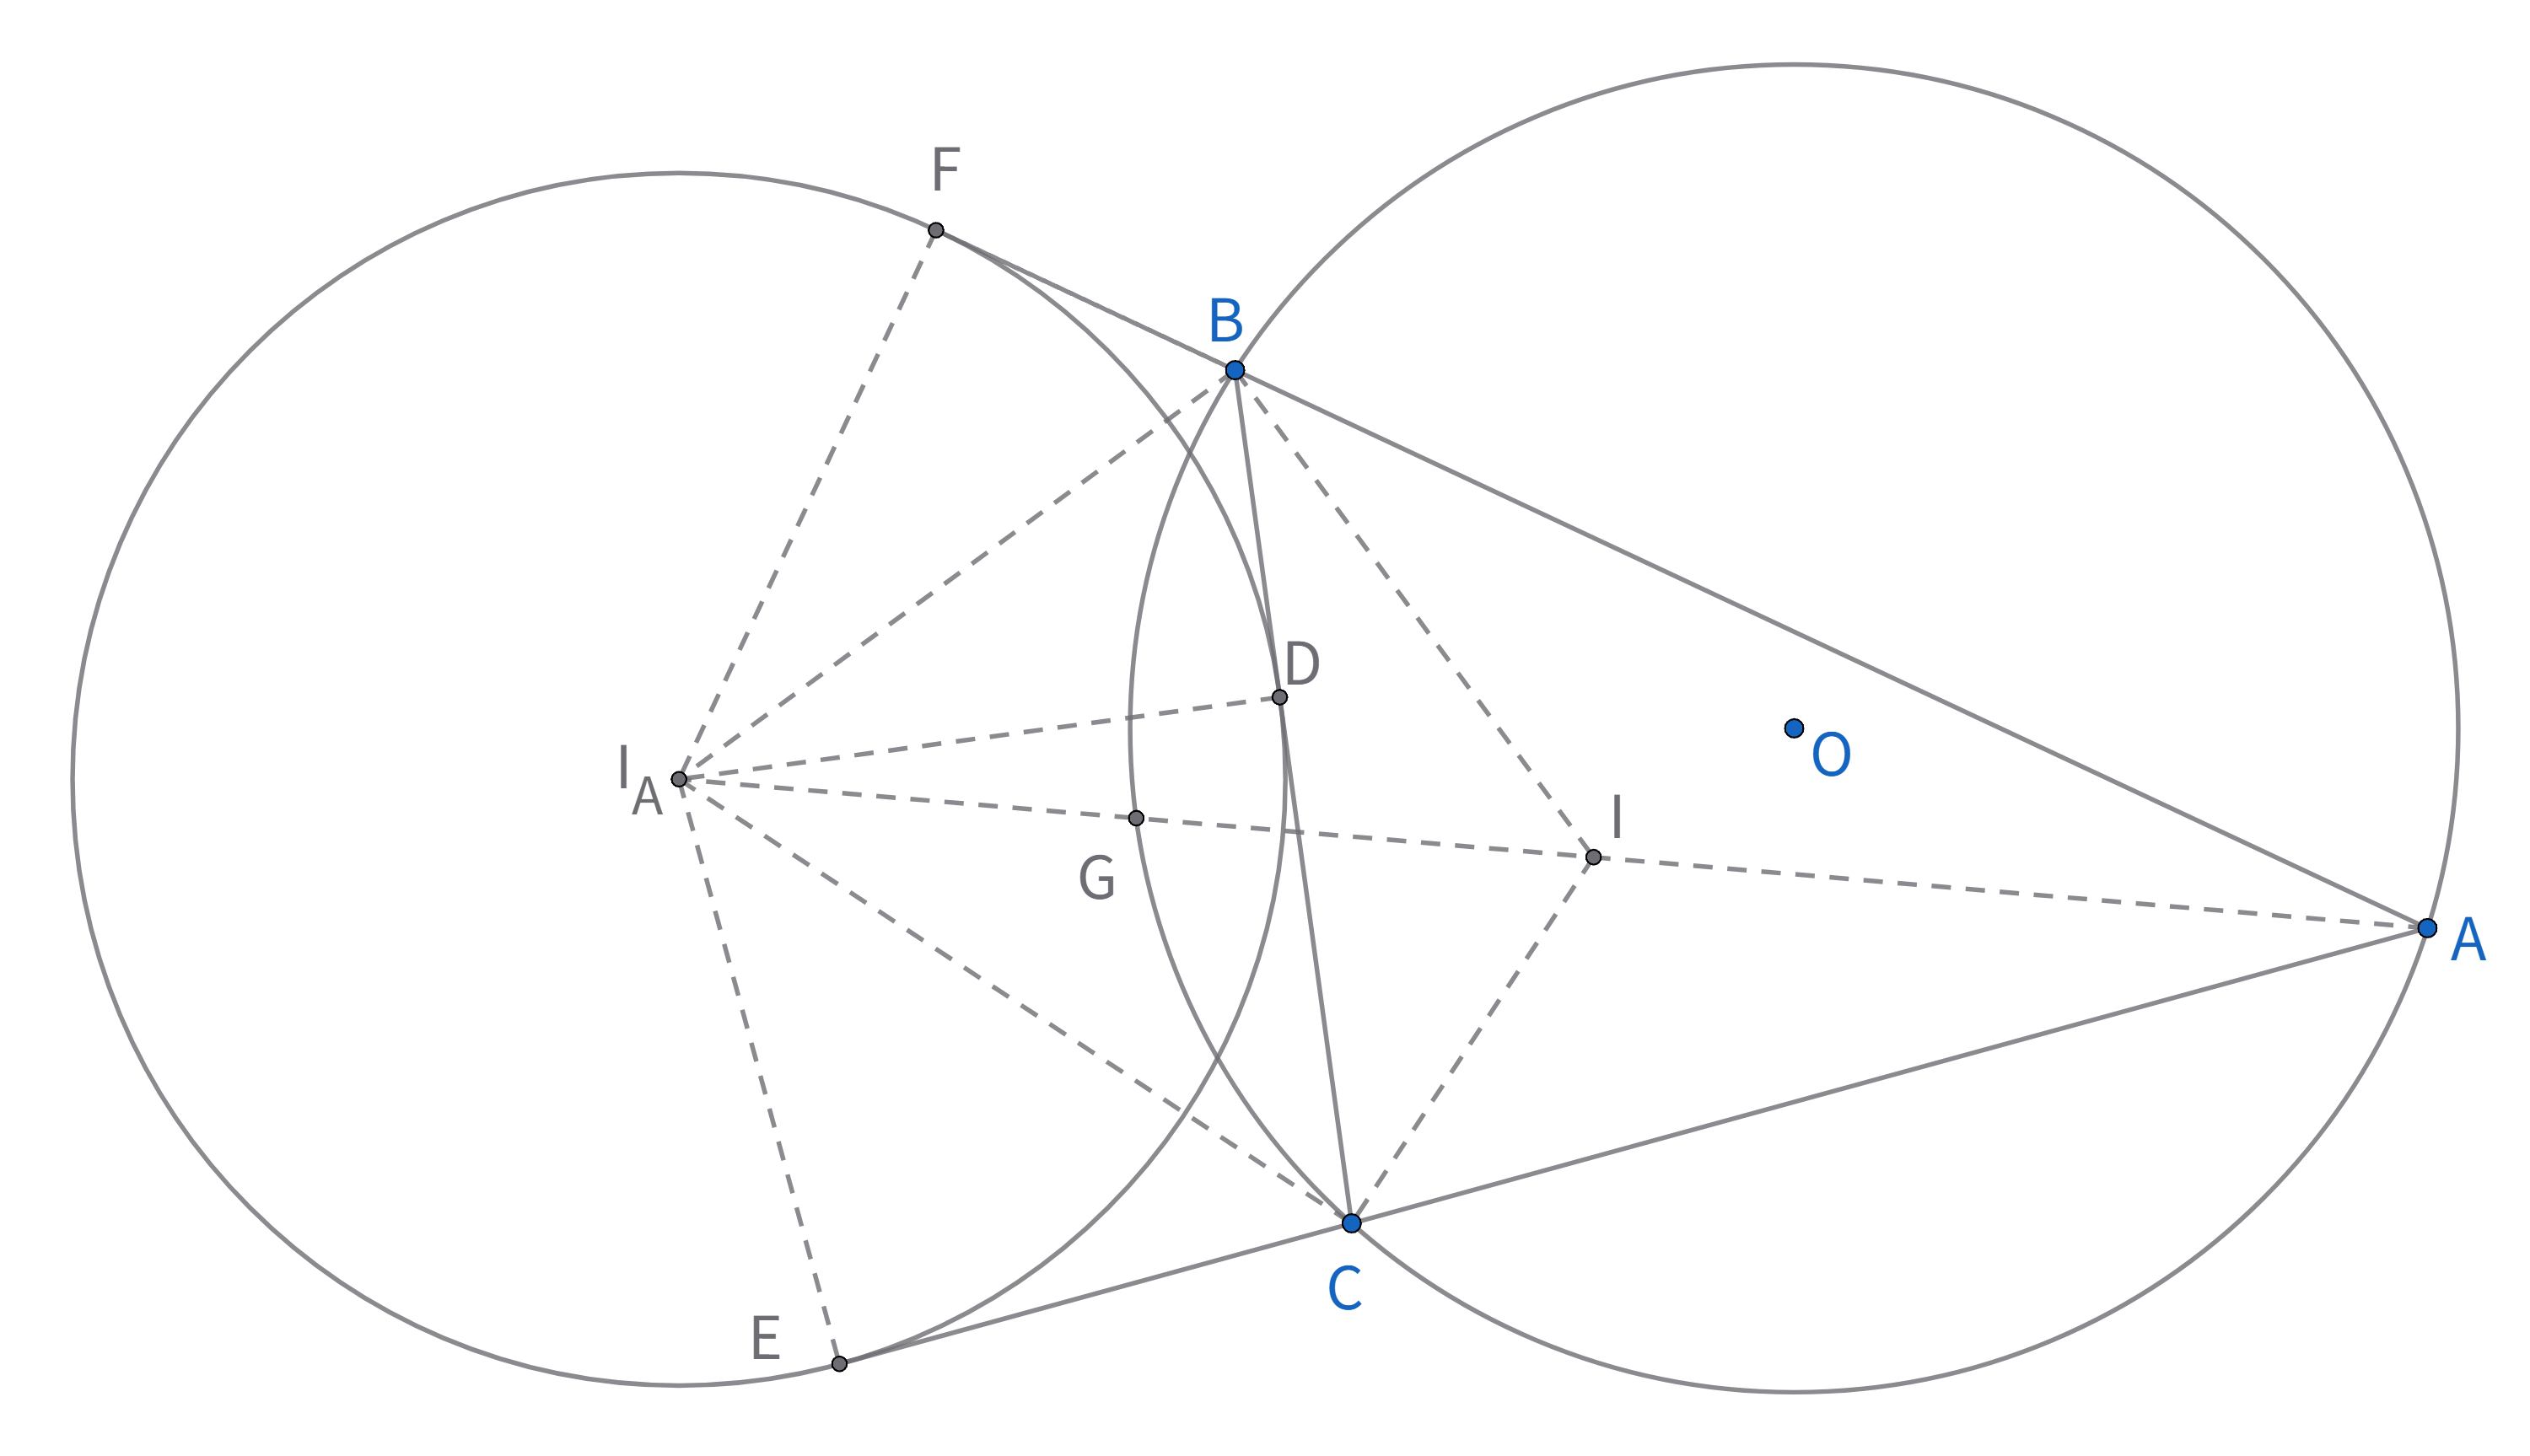
\includegraphics[width=0.6\linewidth]{figures/旁心.png}
    \caption{旁心}
\end{figure}


\begin{proposition}[旁心性质]
    三角形旁心具有如下性质。
    
    (1) 旁心是三角形一内角平分线及其他两角外角平分线的交点。

    (2) 旁心到三角形三边的距离相等。

    (3) $\angle I_ABC = 90^\circ - \frac{1}{2}B, \angle I_ACB = 90^\circ - \frac{1}{2}C, \angle BI_AC=90 - \frac{1}{2}A.$

    (4) $\quad IB\perp BI_A, \quad IC\perp CI_A.$,所以$B, I,C,I_A$四点共圆,且圆心为$\overset{\frown}{BC}$的中点。

    (5) 内心I是旁心三角形$I_AI_BI_C$的垂心。

    (6) 设D、E、F分别为内切圆I在BC、CA、AB上的切点,则定点到旁切圆的切线长度可由三边边长表示:
    $$
    AE=AF=\frac{1}{2}(a+b+c),\quad
    BF=BD=\frac{1}{2}(a+b-c),\quad 
    CD=CE=\frac{1}{2}(a+c - b).
    $$
\end{proposition}
% 设D、E、F分别为旁切圆$I_A$在BC、CA、AB上的切点,那么
%     $$
%     ID \perp BC,\quad 
%     IE \perp AC, \quad 
%     IF \perp AB.$$

\begin{figure}[ht]
    \centering
    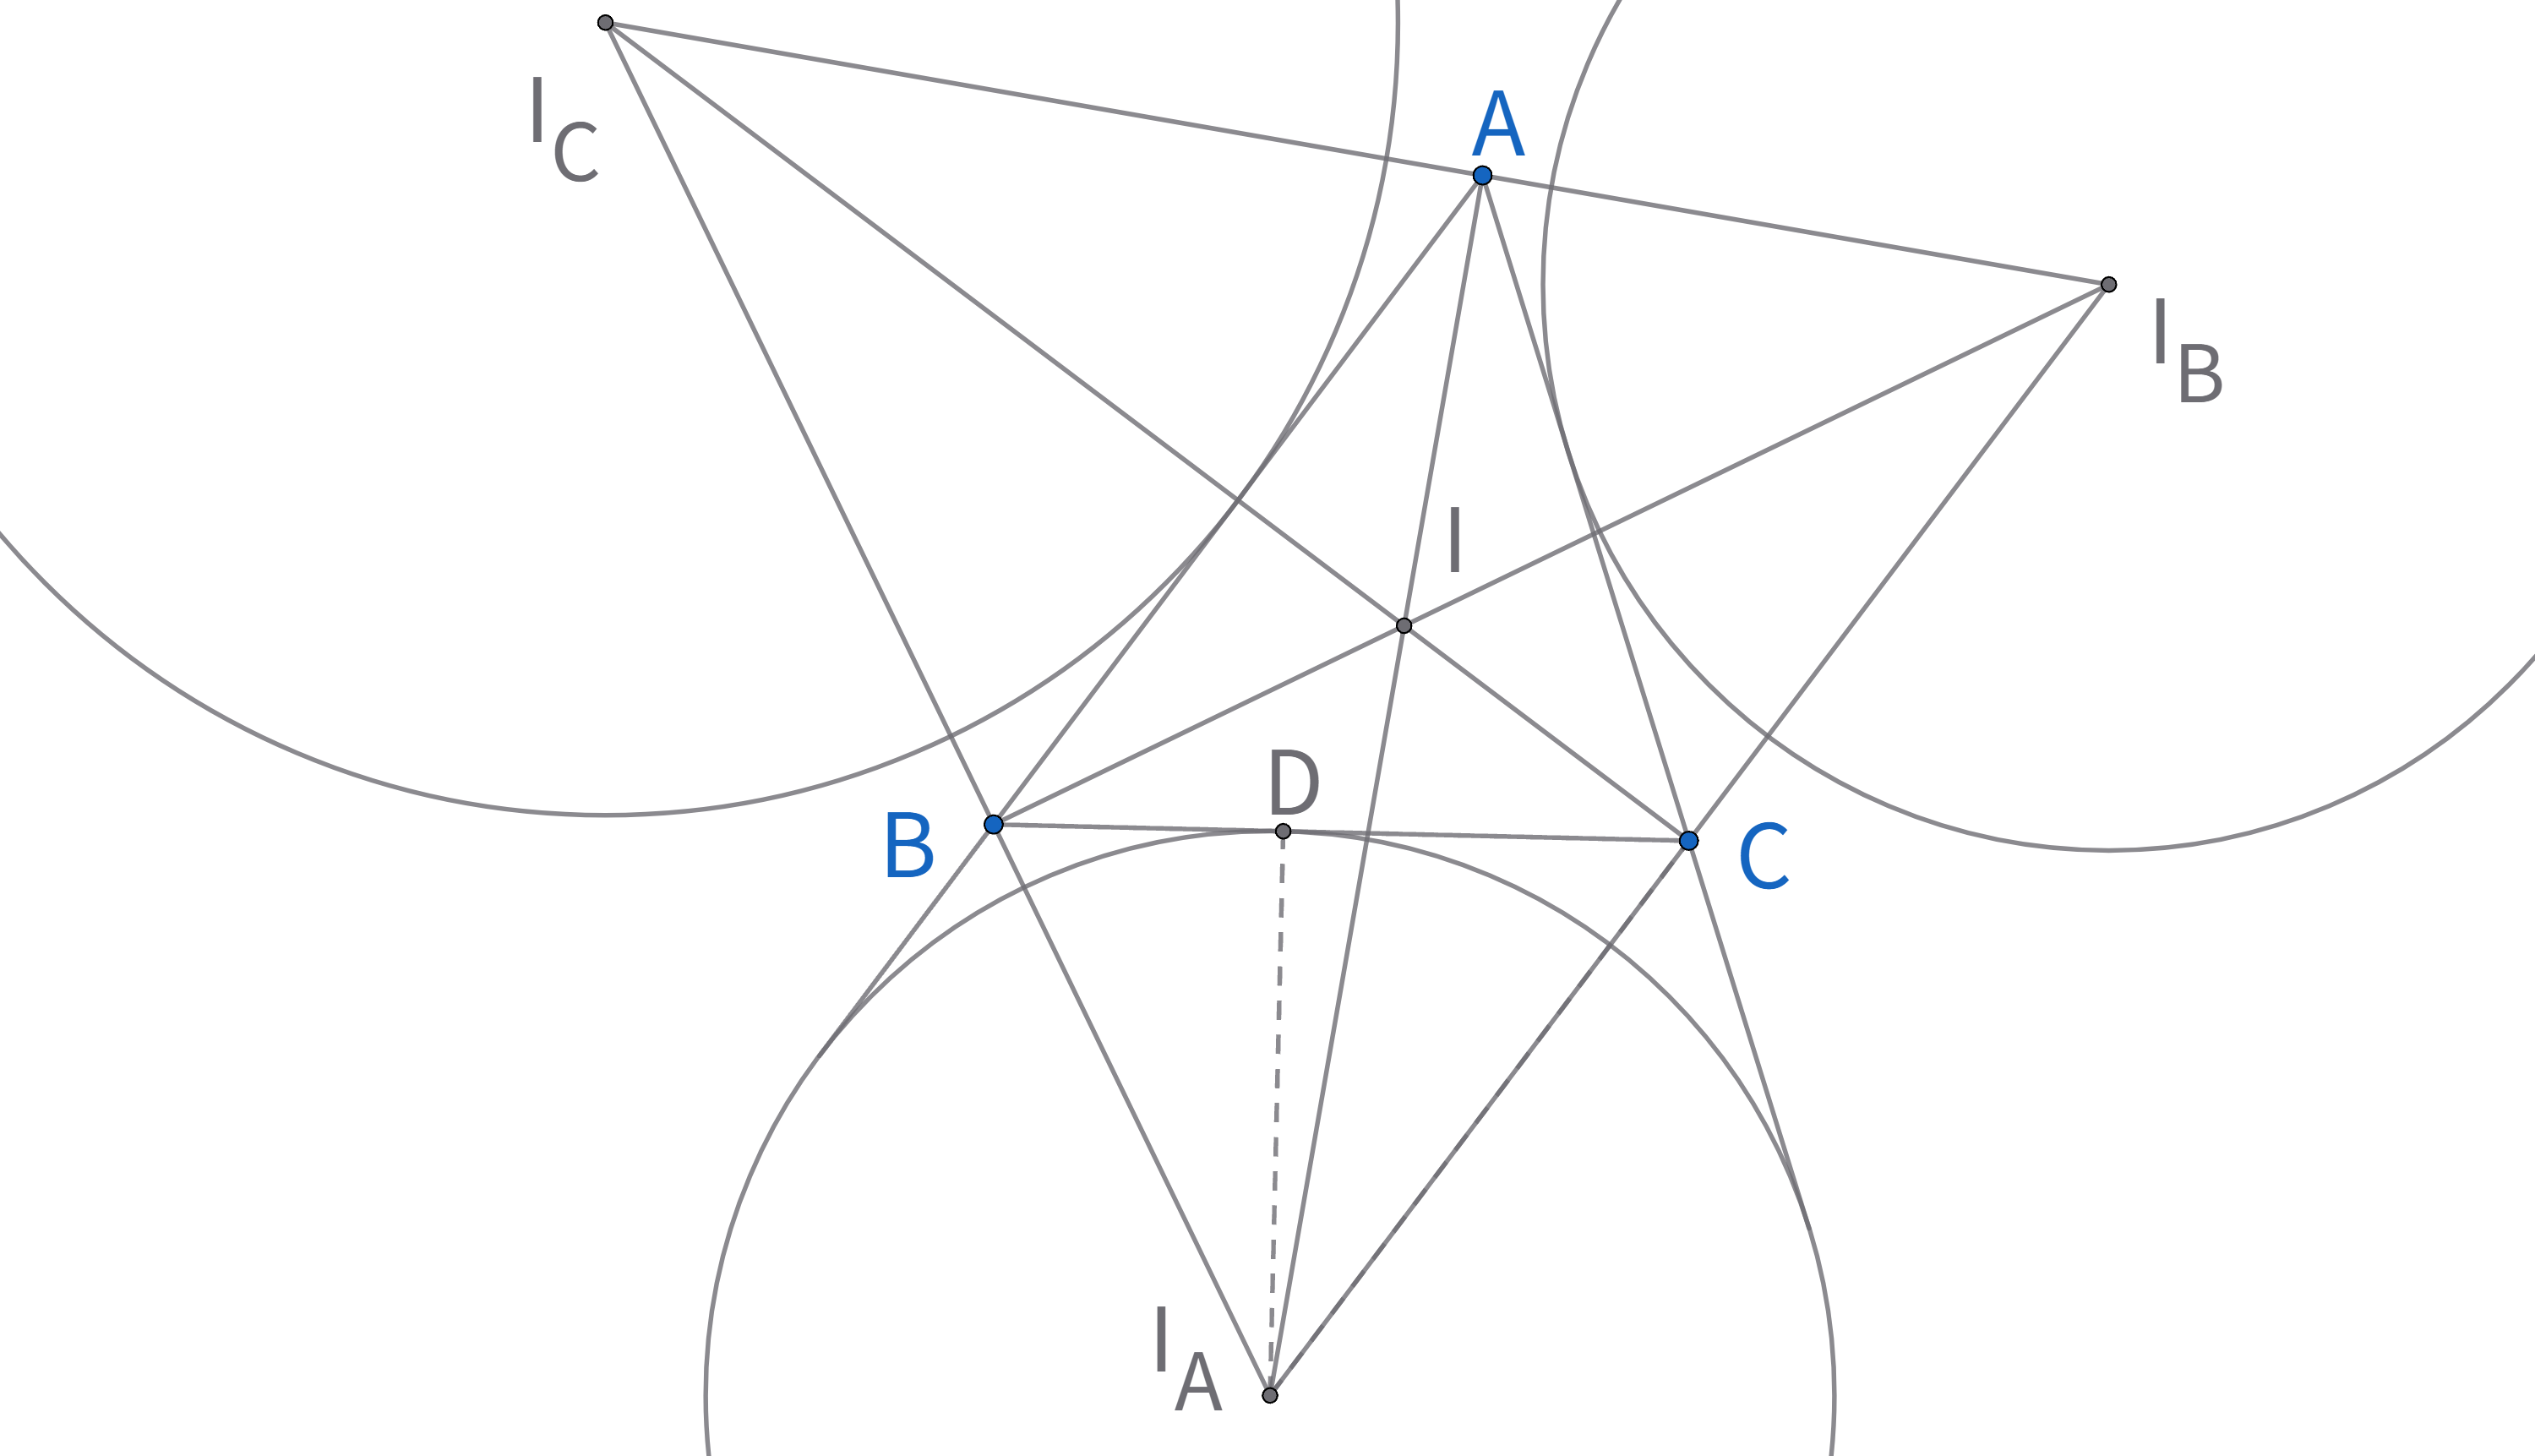
\includegraphics[width=0.4\linewidth]{figures/旁心三角形.png}
    \caption{旁心三角形}
\end{figure}